\documentclass[12pt,a4paper]{article}
\usepackage[utf8]{inputenc}
\usepackage[german]{babel}
\usepackage[T1]{fontenc}
\usepackage{amsmath}
\usepackage{amsfonts}
\usepackage{hyperref}
\usepackage{amssymb}
\usepackage{graphicx}
\usepackage{listings}
\usepackage[left=2cm,right=2cm,top=2cm,bottom=2cm]{geometry}

%if this is changed, check if the url in the first java ref is shown correctly.
\bibliographystyle{alpha}

%configure syntag highlighting
\usepackage{listings}

%dont forget commas at end of every line!!!
\lstset{ 
language=Java,
frame=single,
%bext line shrinks 2 space to 1 so code can be copied from intellij without reformatting
%literate={\ \ }{{\ \ }}1,
breaklines=true,
columns=fullflexible,
numbers=right,
}

%this removes EINRÜCKUNG at text after a figure
\setlength{\parindent}{0pt}

%%this removes empty ":" after abbildung 1:
\usepackage{caption}

\newtheorem{theorem}{Definition}
\author{Frank Leuchtmann}
\title{Systematische Generierung konsistenter Mengen qualitativer
Konditionale}

% this value solves the problem overfull hbox. it defines somehow max empty space in a line.
\tolerance=950

\newcommand{\lag}{\mathcal{L}}

%%the following 2 is to define the dotl command. can this be shorter??
\newcommand\dotl{\mathrel{%
    \mathchoice{\QEQ}{\QEQ}{\QEQ}{\QEQ}%
}}
\def\QEQ{{%
    \setbox0\hbox{<}%
    \rlap{\hbox to \wd0{\hss \raisebox {0.1pt}{$\ \cdot$\hss}}}\box0
}}

\newcommand\dotll{\mathrel{%
    \mathchoice{\QEQQ}{\QEQQ}{\QEQQ}{\QEQQ}%
}}
\def\QEQQ{{%
    \setbox0\hbox{$\leqslant$}%
    \rlap{\hbox to \wd0{\hss \raisebox {1pt}{$\ \cdot$\hss}}}\box0
}}

% rdotl command
\newcommand\rdotl{\mathrel{%
    \mathchoice{\RQEQ}{\RQEQ}{\RQEQ}{\RQEQ}%
}}
\def\RQEQ{{%
    \setbox0\hbox{$\prec$}%
    \rlap{\hbox to \wd0{\hss \raisebox {0.01pt}{$\ \cdot$\hss}}}\box0
}}

\begin{document}
\maketitle
\newpage
\tableofcontents
\newpage
\section{Einleitung}
Diese Arbeit hat zum Ziel, Wissensbasen aus qualitativen Konditionalen auf eine systematische Art und Weise zu generieren. Dafür wird der in \cite{beierle19} entwickelte Algorithmus zur Berechnung aller Wissensbasen implementiert. Dabei soll ergründet werden, welchen Aufwand diese Generierung mit einer steigender Anzahl der darin  enthaltenden Konditionalen verursacht. Die als Ergebnis entstandenen Wissensbasen sollen dann dazu dienen, das System InfOCF (siehe \cite{beierle17}) experimentell zu evaluieren. \\
%descriptionn of parts
Der Ablauf dieser Arbeit ist wie folgt: Ganz am Anfang werden die Grundlagen zu Konditionalen und Wissensbasen kurz dargestellt, um eine Basis für das weitere Vorgehen zu schaffen. Die Aufgabenstellung wird dann in zwei Teilen bearbeitet: Im ersten Teil werden die Konditionale in Normalform berechnet und damit die Menge aller Konditionale $NFC$ gebildet. Anschließend werden auf dieser Menge die Äquivalenzklassen Untersucht und damit die Menge der kanonischen Konditionale $cNFC$ sowie die einzelnen Äquivalenzklassen berechnet. Dabei werden die Konditionale auch nach der Ordnungsrelation $\rdotl$ sortiert. Im zweiten Teil dieser Arbeit findet dann die eigentliche Generierung der Wissensbasen statt. Dazu wird der Algorithmus zur Generierung der Wissensbasen mit Hilfe einer geeigneter Datenverarbeitung implementiert.\\
Für die Bearbeitung der Aufgabe wird eine Java Programm erstellt und dessen Funktionsweise hier beschrieben. Das Programm ist so aufgebaut, dass es die Aufgabenstellung sowohl für die Signatur aus der eigentlichen Aufgabenstellung $\Sigma = \{a,b,c\}$ als auch für eine reduzierte Version mit $\Sigma = \{a,b\}$ bearbeiten kann. Diese reduzierte Version dient einerseits als Hilfestellung zur Bearbeitung der Aufgabe. Zusätzlich zeigt sich dadurch auch die Problemlösung an manchen stellen etwas besser nachvollziehbar.
\section{Grundlagen}
In diesem Abschnitt werden kurz die Grundlagen aufgeführt, auf denen der Hauptteil dieser Arbeit dann basiert. Die Inhalte und Darstellungen sind dabei aus den Kapiteln über Grundlagen aus \cite{beierle19} und \cite{beierle17} übernommen.
\subsection{Notation}
Einzelne Atome, die betrachtet werden, werden mit Kleinbuchstaben wie $a, b, c,...\ $ bezeichnet. Aussagen über diese werden in Form von Großbuchstaben $A, B, C,...$ dargestellt, die Gesamtheit der Sprache wird als $\lag$ bezeichnet. Die Menge der möglichen Welten, die betrachtet werden, wird mit $\Omega$ beschrieben. In einer dieser Welten $\omega \in \Omega$  hat der Ausdruck $\omega \models A$ die Bedeutung, dass $A \in \lag$ in dieser Welt gilt. Des weiteren wird $\neg A$ als $\overline{A}$ und $A \wedge B$ als $AB$ abgekürzt.
\subsection{Konditionale}
Ein Konditional ist ein Zusammenhang aus einer Vorbedingung (Antecedent) und einer Folgerung (Consequence) aus dieser Vorbedingung in der Form \glqq Wenn, A dann B\grqq . Ein qualitatives Konditional ist ein Konditional unter Unsicherheit und entspricht einem Zusammenhang in der Form \glqq Wenn $A$, dann normalerweise $B$\grqq . Dargestellt wird so ein Konditional $r$ unter Unsicherheit im folgenden mit dem Symbol \glqq$|$\grqq \space in der Form $r = ( \lag | \lag)$. Ein Beispiel ist $r = (B|A)$. Das dazugehörige gegenteilige Konditional lautet dann $\overline{r} = (\overline{B}|A)$.\\
Um die Akzeptanz eines unsicheren Konditionals zu bestimmen, werden sie oft im Rahmen von ordinalen Rangfunktionen nach Wolfgang Spohn betrachtet. Mehr dazu auch in diesem Text im  \autoref{sec:wissensbasen}. Vereinfacht gesagt wird ein unsicheres Konditional dann  akzeptiert, wenn es plausibler ist als das dazugehörige gegenteilige Konditional. Beispielsweise $(B|A)$ wird  dann akzeptiert, wenn $A B$ plausibler ist als $A \overline{B}$, siehe dazu auch \cite{isberner14}. \\
Das Konditional unter Unsicherheit in der Form $(B|A)$ teilt dann die Menge möglicher Welten $\Omega$ in drei Teile auf: Welten, die das Konditional bestätigen ($A B$), Welten die es falsifizieren ($A \overline{B}$) und Welten, auf die das Konditional nicht anwendbar ist, weil die Vorbedingung nicht erfüllt ist ($\overline{A}$). Die letztere Möglichkeit wird auch mit $u$ bezeichnet, was als \textit{unknown} gedeutet werden kann. Damit lässt sich das Konditional als Indikatorfunktion einer möglichen Welt $\omega$ wie folgt darstellen:
\[
  (B|A)(\omega)=\begin{cases}
               1 \quad wenn \quad \omega \quad \models AB\\
               0 \quad wenn \quad \omega \quad \models A\overline{B}\\
               u \quad wenn \quad \omega \quad \models \overline{A}
            \end{cases}
\]

\subsection{Äquivalente und triviale Konditionale}
\label{sec:äquivalenz-konditionale}
Äquivalenz für Konditionale $(\equiv)$ soll im weiteren Verlauf dadurch charakterisiert sein, dass zwei äquivalente Konditionale die Menge der möglichen Welten auf die gleiche Art und Weise unterteilen:
\begin{equation}
(B|A)\equiv (B^\prime|A^\prime) \quad gdw. \quad A\equiv A^\prime \quad und \quad AB \equiv A^\prime B^\prime
\end{equation}
Als triviale Konditionale werden solche beschrieben, die keinen Mehrwert bieten, vgl. \cite{beierle19}. Das beinhaltet sowohl sich selbst Erfüllende wie $(A \models A)$ als auch Konditionale, die einfach das Gegenteil eines anderen Konditionals in der Form $(A \models \overline{B})$ darstellen. Solche Konditionale sind bei der weiteren Betrachtung nicht von Interesse und werden daher nicht weiter beachtet.


\subsection{Ordnungsrelation für Konditionale}
\label{sec:ordnungsrelation}
In diesem Abschnitt wird eine Ordnungsrelation für Konditionale definiert, unter der Konditionale später sowohl geordnet bearbeitet als auch gespeichert werden können.
\begin{theorem}[Ordnungsrelation für Zeichen und Mengen](entnommen aus \cite{beierle19}) \ \\
Für eine Ordnungsrelation $\leqslant$ auf meiner Menge $M$ wird dessen Entsprechung für Zeichen als $\leqslant_{lex}$ notiert. Für die geordneten Mengen $S, S^\prime$ mit $S = \{e_1, ..., e_n\}$ und $S^\prime = \{e_{1}, ... , e_{n\prime}\}$ gilt:
\begin{equation}
 S \leqslant_{set} S ^\prime \quad gdw. \quad n<n^\prime, \text{ oder } n = n ^\prime \text{ und } e_1...e_n  \leqslant_{lex}  e_1^\prime ... e_{n^\prime}^\prime
\end{equation}
\label{def:sortierung-konditionale}
\end{theorem}


Bei der Signatur $\Sigma_{abc}$ mit der Ordnungsrelation $a \dotl b \dotl c$ ergibt sich eine Ordnungsrelation für die möglichen Mengen wie folgt: $\{a\} \dotll_{set} \{b\} \dotll_{set} \{c\} \dotll_{set} \{a,b\} \dotll_{set} \{a,c\} \dotll_{set}\{b,c\} \dotll_{set} \{a, b, c\}$. \\
Im weiteren Verlauf wird oft für die Darstellung von Konditionalen eine Notation mittels möglicher Welten verwendet. Dazu wird anstatt von Aussagevariablen die Menge der möglichen Welten aufgeführt, in denen die Aussage gilt. Für eine Aussage $F$ also in der Form $\Omega_F = \{\omega | \omega \models F \}$. Ein vollständiges Beispiel für die Aussage $A\vee\overline{B}\vee\overline{C}$ sieht dann wie folgt aus: \\
$\Omega_{a\vee\overline{b}\vee \overline{c}} = \{abc,ab\overline{c},a\overline{b}c,a\overline{b}\overline{c},\overline{a}b\overline{c},\overline{a}\overline{b}c,\overline{a}\overline{b}\overline{c}\}$ \\
Um diese Notation etwas kompakter darzustellen, wird eine Repräsentation $[[\omega]]_{\dotl}$ für eine mögliche Welt unter der Signatur $\Sigma_{abc}$ per Zahl definiert, angelehnt an deren Interpretation als Binärzahl: \\
$[[abc]]_{\dotl}  = 7,\ 
[[ab\overline{c}]]_{\dotl} = 6,\ 
[[a\overline{b}c]]_{\dotl} = 5,\ 
[[a\overline{b}\overline{c}]]_{\dotl} = 4 ,\
[[\overline{a}bc]]_{\dotl} = 3,\ 
[[\overline{a}b\overline{c}]]_{\dotl} = 2 ,\  
[[\overline{a}\overline{b}c]]_{\dotl}  = 1,\ 
[[\overline{a}\overline{b}\overline{c}]]_{\dotl} = 0 $ \\
Mit dieser Notation sieht das Beispiel von oben wie folgt aus: \\
$\Omega_{a\vee\overline{b}\vee \overline{c}} = \{ 7,6,5,4,2,1,0\}$
\begin{theorem}[Ordnungsrelation für Welten und Konditionale]\ \\(entnommen aus \cite{beierle19})\ \\
Mit einer Signatur $\Sigma$ und deren linearer Ordnung $\dotl$ sind die Ordnungen $\overset{\mathrm{\omega}}{\dotll}$ für Welten $\omega, \omega'$ und $\overset{\mathrm{c}}{\dotll}$ Konditionale $(B|A), (B'|A')$ wie folgt definiert:
\begin{equation}
\omega \overset{\mathrm{\omega}}{\dotll} \omega' \quad gdw. \quad [[\omega]]_{\dotl} \geqslant [[\omega']]_{\dotl}
\end{equation}

\begin{equation}
\label{eq:conditional-order} 
(B|A) \overset{\mathrm{c}}{\dotll} (B'| A') \quad gdw. \quad \Omega_A \overset{\mathrm{\omega}}{\dotll}_{set} \Omega_{A'} \quad oder \quad \Omega_A =  \Omega_{A'} \quad und \quad  \Omega_B \overset{\mathrm{\omega}}{\dotll}_{set} \Omega_{B'}
\end{equation}

\end{theorem}
Da sich die Unterscheidung von $\overset{\mathrm{\omega}}{\dotl}$ und $\overset{\mathrm{c}}{\dotl}$ aus dem Kontext ergibt, wird der Einfachheit halber im weiterem Verlauf $\dotl$ verwendet. \\
Mit der Signatur $\Sigma_{abc}$ ergibt sich für mögliche Welten beispielsweise $abc \dotl ab\overline{c} \dotl \overline{a}bc \dotl \overline{a} \overline{b} \overline{c}$. Ein Beispiel für die Ordnungsrelation für Konditionale ist $(abc|abc \vee ab \overline{c}) \dotl (abc | abc \vee \overline{a} \overline{b} \overline{c} )$ oder $(abc \vee \overline{a} \overline{b} \overline{c} | abc \vee ab \overline{c} \vee \overline{a} \overline{b} \overline{c}) \dotl (\overline{a} \overline{b} \overline{c} |  abc \vee ab \overline{c} \vee \overline{a} bc \vee \overline{a} \overline{b} \overline{c})$.
\subsection{Normalform für Konditionale}
Im Folgenden wird eine Normalform für Konditionale beschrieben. Das Ziel ist die klare Definition einer vollständigen und minimalen  Menge an nichttrivialen Konditionalen über einer Signatur $\Sigma$, die untereinander nicht äquivalent sind. Diese Normalform wird mit $NFC(\Sigma)$ bezeichnet.

\begin{theorem}[Normalform für Konditionale](entnommen aus \cite{beierle19})\\
Die folgende Charakterisierung beschreibt die Menge der Konditionale in Normalform über einer gegebenen Signatur $\Sigma$: \\ \\
$NFC(\Sigma) = \{(B|A)|A \subseteq \Omega_A, B \subsetneq A, B \neq \emptyset \}$ \\ \\
Für diese Menge gelten dann die folgenden drei Eigenschaften:\
 \begin{itemize}
\item{Nichttrivialität: $NFC(\Sigma)$ enthält kein triviales Konditional.}
\item{Vollständigkeit: für jedes nichttriviale Konditional in $\Sigma$ existiert ein äquivalentes Konditional in $NFC(\Sigma)$ }
\item{Minimalität: alle Konditionale in $NFC(\Sigma)$ sind paarweise nicht äquivalent.}
\end{itemize}
\end{theorem}

\subsection{Wissensbasen}
\label{sec:wissensbasen}
Eine endliche Menge $\mathcal{R} \subseteq (\lag | \lag)$ an Konditionalen wird als Wissensbasis bezeichnet. Um die Konsistenz einer Wissensbasis zu untersuchen, werden oft ordinale Rangfunktionen verwendet, welche im Folgenden kurz beschrieben werden. \\
Rangfunktionen wurden von Wolfgang Spohn entwickelt, siehe dazu auch \cite{spohn88} oder \cite{spohn12}. Eine Rangfunktion ist eine Funktion in der Form $\kappa :  \Omega \rightarrow \mathbb{N}_0 $. Mit einer Rangfuntion wird einer Welt $\omega$ aus den möglichen Welten $\Omega$ eine natürliche Zahl mittels einer Funktion $\kappa$ zugeordnet, um deren Grad an Plausibilität zu beschreiben. Mindestens eine Welt bekommt den Wert 0 zugewiesen und wird damit am meisten plausibel gekennzeichnet, weniger plausiblere Welten bekommen aufsteigend entsprechend ihrer Unplausibilität höhere Werte zugeordnet. Mittels solcher Rangfunktionen können sowohl einzelne Aussagen als auch Konditionale betrachtet werden.\\
Rangfunktion für Aussagen:
\[
 \kappa(A)=\begin{cases}
			min\{\kappa(\omega)|\omega \models A \} \quad wenn \  A \ akzeptiert \ wird \\
			\infty \quad andernfalls
            \end{cases}
\]
Rangfunktion für Konditionale:
\[
\kappa((B|A))=\begin{cases}
			\kappa(AB) - \kappa(A) \quad wenn \ \kappa(A) \neq \infty \\
			\infty \quad andernfalls
            \end{cases}
\]
Eine Aussage $A$ wird von einer Rangfunktion akzeptiert, wenn sie plausibler ist und damit einen geringeren Rang besitzt als dessen Gegenteil $\overline{A}$, z.B. $\kappa(A) < \kappa(\overline{A})$. Analaog dazu wird ein Konditional $(B|A)$ akzeptiert, wenn es einen geringeren Rang als dessen gegenteiliges Konditional $(\overline{B}|A)$ besitzt, z.B. $\kappa(AB)<\kappa(A\overline{B})$, vgl. \cite{beierle17}. Eine Wissensbasis $\mathcal{R}$ wird dann als konsistent eingeschätzt, wenn es mindestens eine Rangfunktion gibt, die alle in der Wissensbasis enthaltenen Konditionale akzeptiert.\\

Um konsistente Wissensbasen zu generieren, wird im Algorithmus GenKB der Test auf Toleranz nach \cite{goldszmidt96}S.64 benötigt. Toleranz ist dabei folgendermaßen definiert:
\begin{theorem}[Toleranz eines Konditionals einer Wissensbasis]
\label{def:toleranz}
Ein Konditional $(B|A)$ wird von einer Wissensbasis $\mathcal{R} = {(B_i|A_i)}$ toleriert, wenn eine Welt $\omega$ existiert die $(B|A)$ bestätigt und kein Konditional in $\mathcal{R}$ falsifiziert.
\begin{equation}
\omega \models A \wedge B \bigwedge^n_{i=1}(B_i|A_i)
\end{equation}
\end{theorem}
Ein Konditional $(B|A)$ nicht zu falsifizieren bedeutet in dem Zusammenhang, es entweder zu bestätigen in Form von $A \wedge B$, oder dass die Vorbedingung nicht zutrifft in Form von $\overline{A}$ also zusammengefasst $\overline{A} \vee B$. \\
Mit dieser Definition von Toleranz kann nun die Konsistenz einer Wissensbasis definiert werden (siehe \cite{goldszmidt96}).
\begin{theorem}[Konsistenz einer Wissensbasis]
\label{def:konsistenz}
Eine Wissensbasis $\mathcal{R}$ ist konsistent gdw. für jede nicht leere Teilmenge $\mathcal{R}' \subseteq \mathcal{R}$ ein Konditional existiert welches von $\mathcal{R}'$ toleriert wird.
\end{theorem}
Aus dieser Defintion entsteht dann der folgende Algorithmus zum Testen einer Wissensbasis auf Konsistentz, ebenfalls entnommen aus \cite{goldszmidt96}. \\

Input: A knowledge base $\mathcal{R}$ \\
Output: An ordered partition $\mathcal{R} = (\mathcal{R}_o, \mathcal{R}_1, ...,  \mathcal{R}_k)$ if $\mathcal{R}$ is consistent \\
%mathescape = true makes $$ work in here
\begin{lstlisting}[mathescape=true]
1: i = 0
2: while $\mathcal{R}$ is non-empty
	a)Find the set of rules $\mathcal{R}_i$ from $\mathcal{R}$ such that each conditional from it is tolerated by $\mathcal{R}$
	b: if none can be found: abort, $\mathcal{R}$ is iconsistent
	c: else remove $\mathcal{R}_i$  from $\mathcal{R}$ and set i = i + 1
3: return the ordered partition $\mathcal{R} = (\mathcal{R}_o, \mathcal{R}_1, ..., \mathcal{R}_k)$
\end{lstlisting}


Als nächstes wird noch kurz die Äquivalenz von Wissensbasen betrachtet. Diese ist bei der Generierung von Wissensbasen von Bedeutung, um neue Wissensbasen und syntaktische Varianten bereits vorhandener Wissensbasen unterscheiden zu können. Als Maßstab für Äquivalenz zweier Wissensbasen wird im folgenden die elementweise Äquivalenz verwendet. Diese verfolgt den Grundgedanken, dass Teile einer Wissensbasis mit Teilen von anderen Wissensbasen einzeln verglichen werden können.
\begin{theorem}[Elementweise Äquivalenz von Wissensbasen] \ \\(entnommen aus \cite{beierle17b}) \ \\
$\mathcal{R}$ und $\mathcal{R'}$ sind Wissensbasen. Für diese gilt dann:
\begin{itemize}
\item{$\mathcal{R}$ ist eine elementweise äquivalente untergeordnete ($\ll_{ee}$) Wissensbasis von $\mathcal{R'}$ gdw. für jedes Konditional $(B'|A') \in \mathcal{R'}$, welches nicht selbsterfüllend ist, ein Konditional $(B|A) \in \mathcal{R}$ existiert, sodass gilt $(B|A) \equiv (B'|A')$.}
\item{$\mathcal{R}$ und $\mathcal{R'}$ sind strikt elementweise äquivalent gdw. $\mathcal{R} \ll_{ee} \mathcal{R'}$ und $\mathcal{R}' \ll_{ee}\mathcal{R}$.}
\item{$\mathcal{R}$ und $\mathcal{R'}$ sind elementweise äquivalent ($\mathcal{R} \equiv_{ee} \mathcal{R'}$) gwd. $\mathcal{R}$ und $\mathcal{R'}$ entweder inkonsistent oder strikt elementweise äquivalent sind.}
\end{itemize}
\end{theorem}
\subsection{Isomorphie und Äquivalenzklassen}
\label{sec:äquivalenz-wissensbasen}
Durch Umbenennung von Variablen ist es möglich, neue Kombinationen von Welten, Konditionalen oder Wissensbasen zu schaffen, die sich außer dieser Umbenennung nicht von den bereits Vorhandenen unterscheiden. Dieses Verhalten wird als Isomorphismus beschrieben. Die Menge der durch Isomorphie ineinander umwandelbaren Dinge wird als Äquivalenzklasse bezeichnet. \\
Beispielsweise enthält die Signatur $\Sigma_{abc}$ die mögliche Kombination $\overline{a}bc$. Wenn jetzt $a$ in $b$ und $b$ in $a$ umbenannt wird, entsteht der Isomorphismus $a\overline{b}c$. Analog kann durch Umbenennung von $a$ und $c$ daraus $ab\overline{c}$ entstehen. Alle drei bilden zusammen eine Äquivalenzklasse. Entsprechend ergibt sich die folgende Definition.
\begin{theorem}[Isomorphismus](entnommen aus \cite{beierle19}) \ \\
$X, X'$ sind Welten, Aussagen, Wissensbasen oder Mengen dieser Dinge. $X$ und $X'$ sind dann isomorph $(X \simeq X')$, wenn eine Umbenennung in der Form $\rho(X) = X'$ existiert.
\end{theorem}
Für die Signatur $\Sigma_{abc}$ ergeben sich dann die folgenden vier Äquivalenzklassen: \\
$[\Omega_{\Sigma abc}]_{/\simeq}=\{[abc]$, $[ab\overline{c}, a\overline{b}c\, \overline{a}bc], [a\overline{b}\overline{c}, \overline{a\\}b\overline{c}, \overline{a}\overline{b}c], [\overline{a}\overline{b}\overline{c}]\}$ \\
Die Menge der Äquivalenzklassen in einer Menge $M$ mit dem Element $m \in M$ wird im Folgenden mit $[M]_{/\equiv}$ und die konkrete Äquivalenzklasse welche $m$ enthält mit $[m]_\equiv$ notiert.\\
Mit Berücksichtigung von Äquivalenzklassen und der Ordnung $\dotl$ aus \autoref{sec:ordnungsrelation} wird in der nächsten Definition eine Ordnungsrelation konstruiert, die diese Äquivalenzen mit einbezieht.


\begin{theorem}[$cNFC(\Sigma)$ $und$ $Ordnungsrelation$ $\rdotl$](entnommen aus \cite{beierle19}) \ \\
Gegeben sei eine Signatur $\Sigma$ mit der linearen Ordnung $\dotl$. Dann sind $[NFC(\Sigma)]_{/ \simeq}=\{[r_1]_\simeq,...,[r_m]_\simeq\}$ die Äquivalenzklassen von $NFC(\Sigma)$ induziert durch Isomorphismus. Für jedes $i \in \{1, ..., m\}$ ist dann das Konditional $r_i$ das minimale Element in $[r_i]_\simeq$ im Sinne von $\dotl$ ist und $r_1\dotl...\dotl r_m$.
\begin{itemize}
\item{Die kanonischen Konditionale in Normalform über $\Sigma$ sind $cNFC(\Sigma) = \{r_1, ..., r_m \}$.}
\item{Die kanonische Ordnung auf $NFC(\Sigma)$ ($\rdotl)$ ist durch folgendes Schema gegeben: \\
$r_1\rdotl ... \rdotl r_m \rdotl[r_1]_\simeq \setminus \{r_1\} \rdotl ... \rdotl [r_m]_\simeq \setminus \{r_m\}$ \\ 
mit $r \rdotl r'$ gdw. $r\dotl r'$ für alle $i \in \{1, ..., m\}$ und alle $r, r' \in [r_i]_\simeq \setminus \{r_i\}$.}
\end{itemize}
\label{def:sortierung-nfc}
\end{theorem}


\section{Überblick auf das erstellte Programm}


\subsection{Voraussetzungen}
Das beschriebene Programm zum Generieren von Wissensbasen ist komplett in Java geschrieben und erfordert zur Benutzung Java in der Version 1.8 oder höher. Neben der von Java standardmäßig mitgebrachten Bibliotheken werden keine weiteren  Abhängigkeiten benötigt. Die verwendete Java Version hat einen Einfluss auf die Geschwindigkeit des Programms: Beispielsweise war es auf dem Test PC mit Java 13 etwa 10$\%$ schneller als mit Java 1.8.


\subsection{Benutzung des Programms}
Das Programm ist leicht zu benutzen, es bringt für alle Funktionen eine GUI mit. Zum Starten führt man einfach die Datei \textit {Conditionals.jar} aus. Beim Starten des Programms ohne explizite Optionen für die JVM bekommt es automatisch einen vom Arbeitsspeicher des PCs abhängigen maximal verwendbaren Arbeitsspeicher zugewiesen. Wenn mit dem Programm keine sehr speicherintensiven Aktionen ausgeführt werden sollen, reicht das vermutlich aus. Es ist ansonsten auch möglich, dem Programm eine benutzerdefinierte maximale Menge an Arbeitsspeicher zuzuweisen. Dazu startet man die Conditionals.jar .jar mit folgendem Konsolenbefehl: 

\begin{lstlisting}
java -Xmx12G -jar Conditionals.jar 
\end{lstlisting}

So legt der erste Parameter die Menge an maximal durch die JVM nutzbaren Arbeitsspeicher fest, hier im Beispiel sind das 12 GB. \\
Wenn das Programm gestartet wurde, öffnet sich ein kleines Fenster. Darin kann der Benutzer dann  auswählen, ob er Konditionale betrachten oder Wissensbasen generieren will.



\subsection{Aufbau des Programms}
In \autoref{pic:overview} ist ein Gesamtüberblick auf das erstelle Programm zu sehen. Die drei Elemente die sich im grau hinterlegten Bereich befinden sind für das generieren der Wissensbasen zuständig. Oben rechts ist die GUI abgebildet. Sie dient zum setzen von Optionen, Starten des Programms und während der Laufzeit zum Anzeigen von verschiedenen Informationen zum Programmablauf. Unten links befindet sich der NfcCreator, hier werden die Konditionale NFC anhand der eingestellten Optionen erstellt. Diese Konditionale werden dann an den KbCreator übergeben, welcher für die eigentliche Generierung der Wissensbasen zuständig ist.  Die GUI oben links NfcViewer ist optional und kann genutzt werden um die Konditionale nach verschiedenen Optionen zu erzeugen, zu betrachten und zu speichern.
\begin{figure}
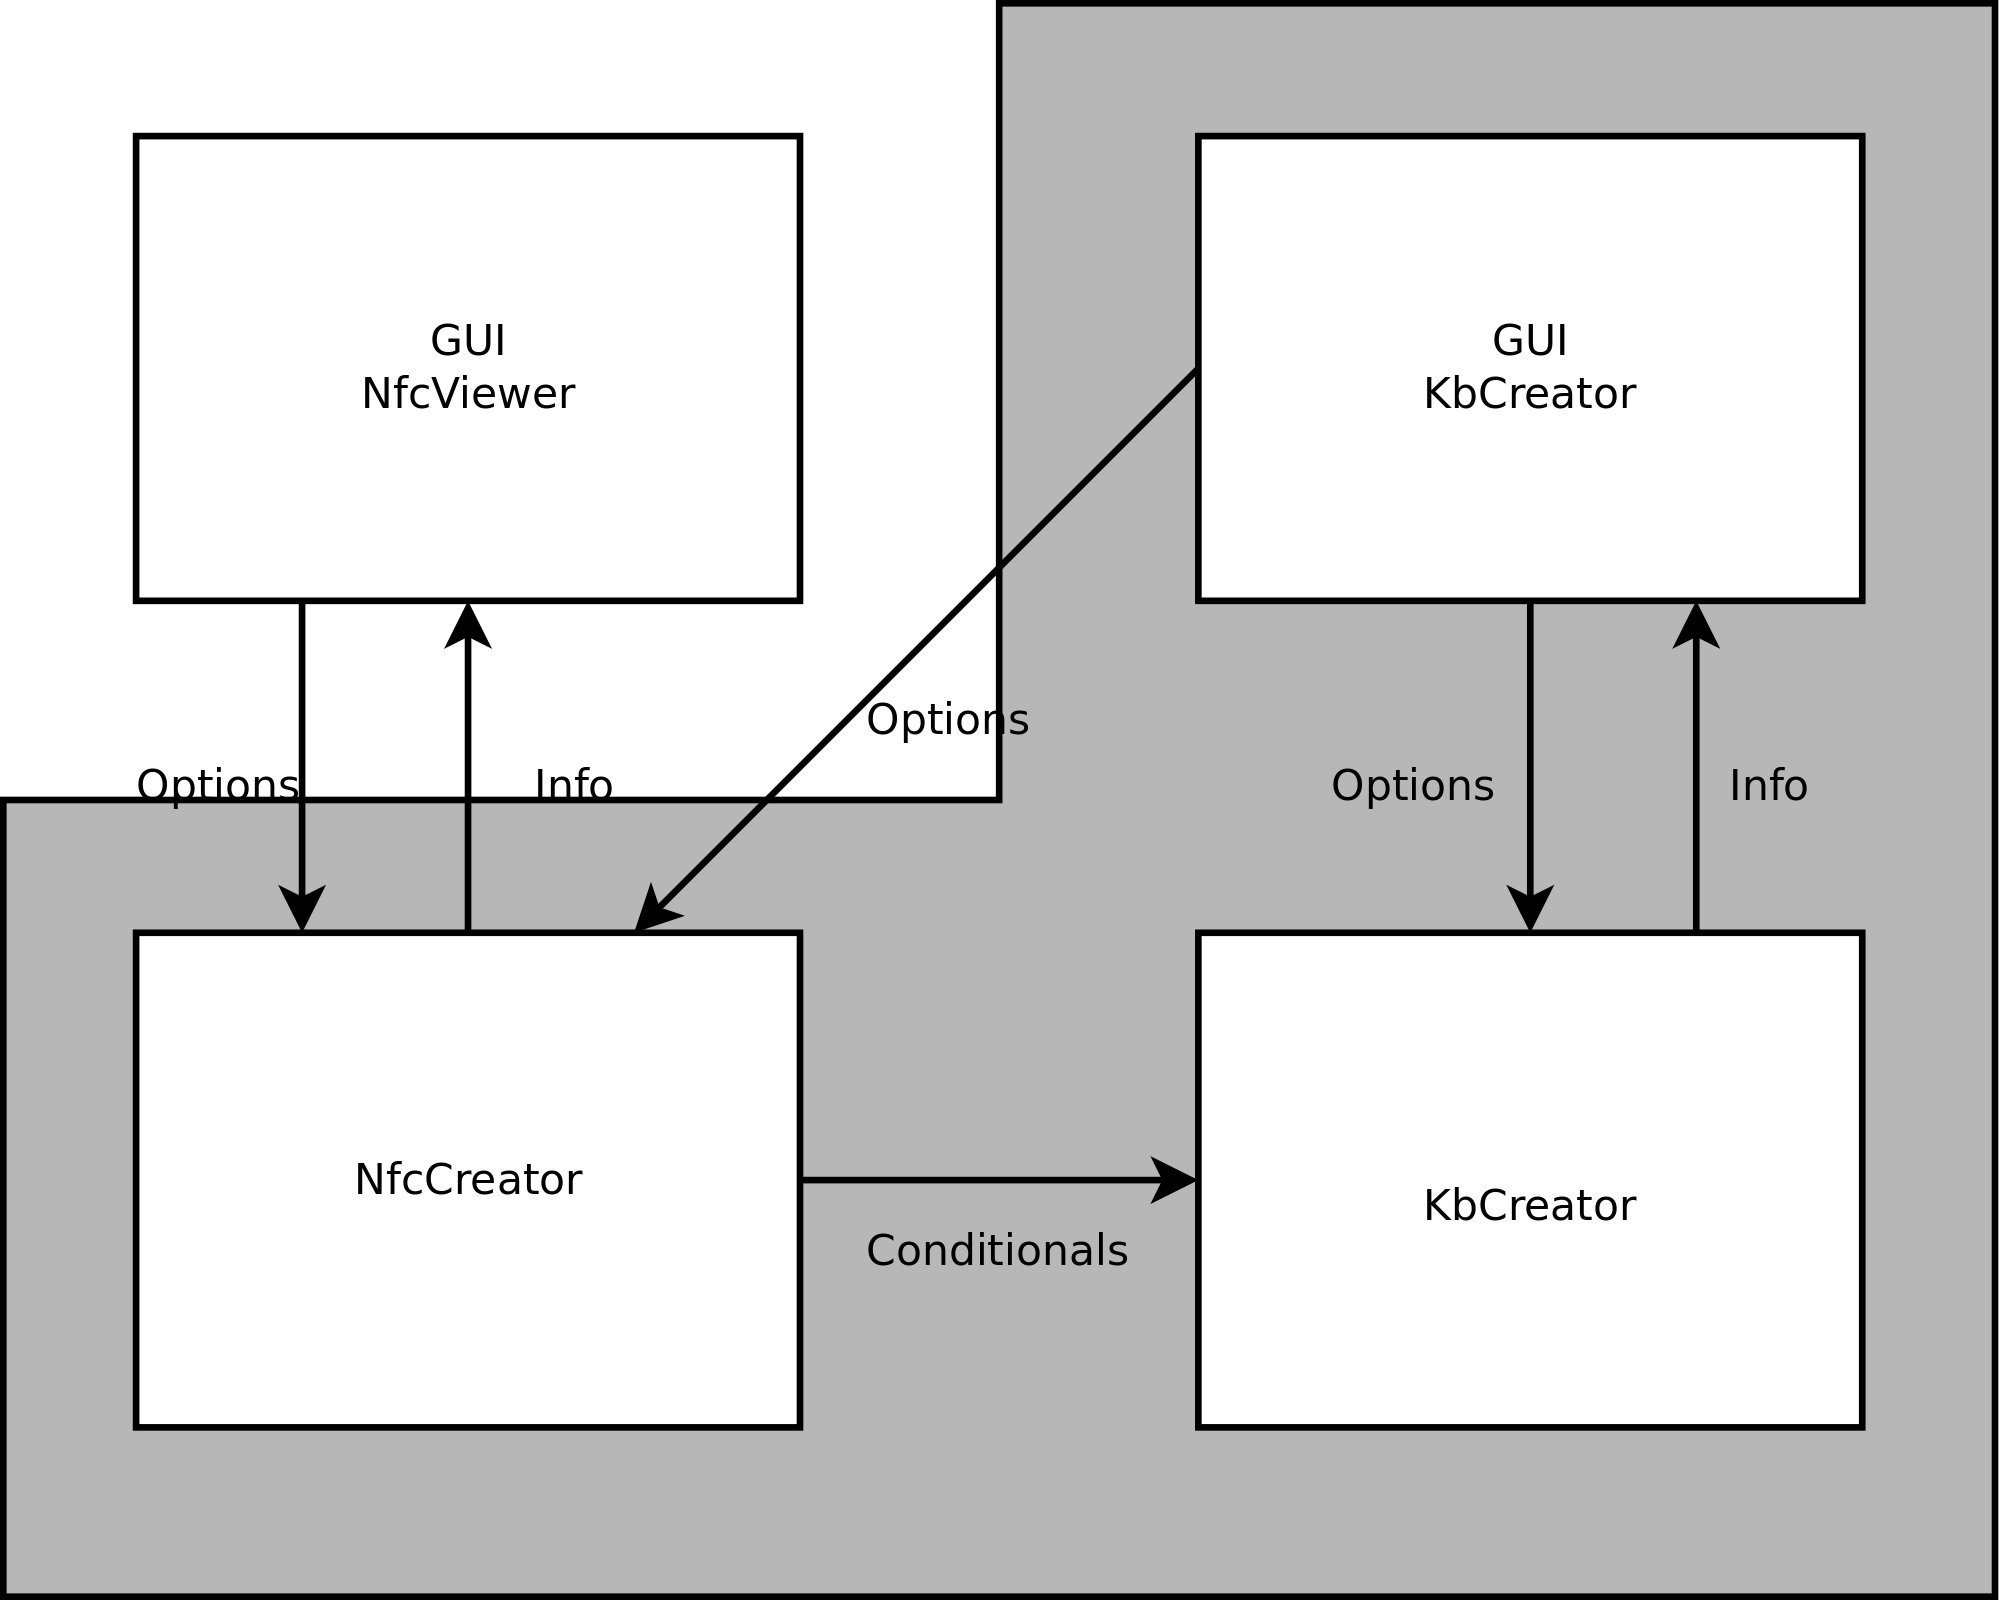
\includegraphics[width=0.7\linewidth]{bilder/overview.png}

\caption{Gesamtübersicht über das erstellte Programm}
\label{pic:overview}
\end{figure}


Der weitere Ablauf der Arbeit ist wie folgt: Im nächsten Abschnitt wird die Berechnung der Konditionale beschrieben, also der Teil aus der Gesamtübersicht, welcher sich unter \glqq NfcCreator\grqq \space verbirgt. Im Anschließenden Teil wird dann die Berechnung der Wissensbasen aus den Konditionalen dargestellt, das ist der Teil, der sich in der Abbildung unter \glqq KbCreator \grqq \space befindet. Anschließend werden die Ergebnisse noch kurz eingeordnet.

\section{Berechnung der Konditionale}

\subsection{Berechnung der Konditionale in Normalform}

In diesem Abschnitt wird beschrieben, wie das erste Teilproblem, die Berechnung der Konditionale und deren Gruppierung in Äquivalenzklassen, gelöst wird. Dazu wurde ein Programm namens \textit{NfcCreator} erstellt. Durch das Berechnen der Konditionale dient das Programm dann als Grundlage für den Hauptteil dieser Arbeit, die Wissensbasen aus den Konditionalen zu erzeugen. Zusätzlich gibt für den NfcCreator noch eine kleine GUI, um die Konditionale mit verschiedenen Optionen erzeugen und betrachten zu können. Diese GUI wird am Ende dieses Abschnitts gezeigt. \\
In den folgenden Unterabschnitten wird die Berechnung der Konditionale in Normalform dargestellt. Dazu wird zuerst die Menge der möglichen Welten berechnet und daraus dann die Menge der Konditionale gebildet. Anschließend werden diese geordnet und in Äquivalenzklassen gruppiert.


\subsubsection{Mengen möglicher Welten}
\label{sec:worldslist}
Die Darstellung der möglichen Welten wurde in \autoref{sec:ordnungsrelation} schon gezeigt, an diesem Punkt setzt die Betrachtung hier an. Wie bereits beschrieben lassen sich aussagenlogische Ausdrücke auch als Mengen möglicher Welten ausdrücken. Diese Form wird zur Darstellung der Normalform für Konditionale verwendet. Eine solche Menge möglicher Welten wird im Folgenden mit einem Objekt der Klasse WorldsList dargestellt. Objekte der Klasse WorldsList repräsentieren später in den Konditionalen dann Antecedent und Consequence. Die Gesamtheit aller solcher möglicher Mengen einer Signatur bestimmt dann die Menge der möglichen Konditionale, die über einer Signatur gebildet werden können. Der Algorithmus, der alle Teilmengen aus den enthaltenen Welten einer Signatur berechnet, ist in \autoref{code:subsets} dargestellt. Als Input wird die Liste möglicher Welten der Signatur verwendet, der Output ist eine Liste aller Teilmengen des Inputs ohne der leeren Menge. \\
Für die Signatur $\Sigma_{abc}$ ergeben sich damit 255 verschiedene Mengen von Welten. (Vergleich: für $\Sigma_{ab}$ sind es 15) Diese können mit dem NFC-Viewer mit dem Button \glqq WORLDS\grqq \space dargestellt werden. Repräsentiert werden diese Mengen von Welten im Programm jeweils durch eine Instanz der Klasse WorldsList, von der ein vereinfachtes Diagramm in \autoref{pic:worldslist} gezeigt ist. 


\begin{figure}
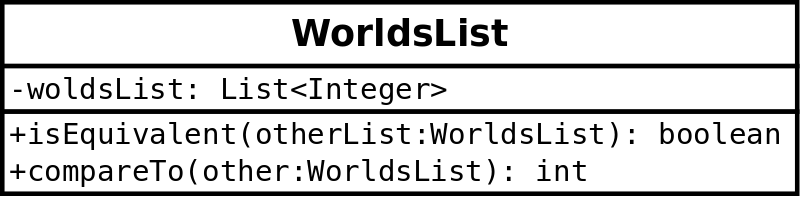
\includegraphics[width=0.45\linewidth]{bilder/worldslist.png}
\caption{WorldsList}
\label{pic:worldslist}
\end{figure}


Das wichtigste Attribut der Klasse WorldsList ist die Liste der möglichen Welten in Form einer \textit{List<Integer>}. Die Klasse WorldsList selbst implementiert das Java Interface \textit{Comparable} und kann damit Objekte erzeugen, die standardisiert untereinander sortiert werden können. Entsprechend besitzt die Klasse die Methode \textit{compareTo(Object o)} zur Sortierung gemäß \autoref{def:sortierung-konditionale}. Dazu vergleicht das Objekt sich selbst mit einem Anderen (dieser Klasse) und gibt als Rückgabewert -1 zurück, wenn das aktuelle Objekt (\textit{this}) kleiner als das Übergebene ist, 0 wenn sie gleich sind und 1 wenn das aktuelle Objekt größer als das übergebene Objekt ist. Die Implementierung der \textit{compateTo(Object o)} Methode ist in \autoref{code:compare-worldslist} dargestellt. Das Interface  \textit{Comparable} und \textit{compareTo(Object o)} wird ähnlich wie hier später auch in anderen Klassen verwendet um die Sortierung von Objekten zu ermöglichen.



\begin{figure}
\begin{lstlisting}
private List<WorldsList> createSubSetList(List<Integer> inputList){
    List<WorldsList> subSetList = new ArrayList<>();
    for (Integer world : inputList) {
        for (ListIterator<WorldsList> setsIterator = subSetList.listIterator(); setsIterator.hasNext(); ) {
            WorldsList newWorld = new WorldsList();
            newWorld.addList(setsIterator.next().getWorldsList());
            newWorld.addInt(world);
            setsIterator.add(newWorld);
        }
        WorldsList otherWorld = new WorldsList();
        otherWorld.addInt(world);
        subSetList.add(otherWorld);
    }
    return subSetList;
}
\end{lstlisting}
\caption{Algorithmus zur Erstellung aller Teilmengen einer Liste möglicher Welten}
\label{code:subsets}
\end{figure}



\begin{figure}
\begin{lstlisting}
public int compareTo(Object o) {
    WorldsList otherWorld = (WorldsList) o;
    if (worldsList.size() < otherWorld.getWorldsList().size())
        return -1;
    if (worldsList.size() > otherWorld.getWorldsList().size())
        return 1;
          
      for (int i = 0; i < worldsList.size(); i++) {
        if (worldsList.get(i) > otherWorld.getWorldsList().get(i))
            return -1;
        if (worldsList.get(i) < otherWorld.getWorldsList().get(i))
            return 1;
    }
    return 0;
}
\end{lstlisting}
\caption{Implementierung compareTo(Object o) der Klasse WorldsList}
\label{code:compare-worldslist}
\end{figure}

Weiterhin besitzt die Klasse WorldsList die Methode \textit{createRenamings()}, welche eine wichtige Rolle für das spätere Finden von äquivalenten Konditionalen besitzt. Wie bereits in \autoref{sec:äquivalenz-konditionale} beschrieben entsteht Äquivalenz von Konditionalen durch Umbenennung von Variablen und besteht somit aus äquivalenten Formeln für Antecedent und Consequence. Entsprechend ergibt sich aus der Menge der möglichen Umbenennungen die Menge sowohl an Formeln als auch an Konditionalen innerhalb einer Äquivalenzklasse. Mit Signatur $\Sigma_{ab}$ existiert eine einzige mögliche Umbenennung, nämlich wenn $a$ in $b$ und $b$ in $a$ umbenannt wird. Mit der Signatur $\Sigma_{abc}$ existieren drei mögliche Umbenennungen durch den Tausch der folgenden Paare an Variablen: $a-b$, $a-c$ und $b-c$. Die Methode \textit{createRenamings()} gibt nun in Abhängigkeit von der gewählten Signatur alle möglichen Umbenennungen einer WorldsList als neue List<WorldsList> in der oben genannten Reihenfolge wieder. Bei nur einer existierenden Umbenennung mit $\Sigma_{ab}$ stellt sich die Frage nach der Reihenfolge offensichtlich nicht, bei $\Sigma_{abc}$ ist diese Reihenfolge später noch wichtig.
\begin{figure}
\begin{lstlisting}
List<Integer> intList = new ArrayList<>(worldsList.size());
for (int world : worldsList) {
    switch (world) {
        case 0:
            intList.add(0);
              break;
        case 1:
            intList.add(1);
              break;
        case 2:
            intList.add(4);
            break;
        case 3:
            intList.add(5);
            break;
        case 4:
            intList.add(2);
            break;
         case 5:
            intList.add(3);
            break;
        case 6:
            intList.add(6);
            break;
        case 7:
            intList.add(7);
            break;
        default:
            throw new RuntimeException("Finding equivalent WorldsList failed!");
    }
}
WorldsList worldsList = new WorldsList();
worldsList.addList(intList);
renamingsList.add(worldsList);
\end{lstlisting}
\caption{Beispiel der Implementierung einer Umbenennung in der Methode \textit{createRenamings} für die Umbenennung $a-b$ in der Klasse WorldsList}
\label{code:renaming}
\end{figure}


Im Folgenden wird nun die Methode \textit{createRenamings()} der Klasse WorlsList genauer erklärt. Das Wesen einer Umbenennung einer WorldsList ist es, dass sich die enthaltene Liste der Welten ändert. Es wird für eine Umbenennung also ein neues Objekt der Klasse WorldsList mit einer neuen List<Integer> Liste der möglichen Welten erstellt. Bei jeder möglichen Umbenennung ändern sich die enthaltenen möglichen Welten auf die selbe Weise, entsprechend wird die ursprüngliche List<Integer> Liste der Welten nach einem charakteristischem Schema \glqq übersetzt\grqq. So ein Schema existiert für jede mögliche Umbenennung, entsprechend gibt es für $\Sigma_{ab}$ eines und für $\Sigma_{abc}$ drei davon. Da der Code für alle Umbenennungen viel Platz benötigt wird hier nicht die ganze Methode \textit{createRenamings} dargestellt. In \autoref{code:renaming} ist beispielhaft die Umbenennung $a-b$ mit der Signatur $\Sigma_{abc}$ gezeigt. In Zeile 1 wird die neue List<Integer> erstellt, in die die übersetzten Werte mit einer Switch Anweisung eingetragen werden. Man sieht, dass sich  Welt 0 $(!a!b!c)$ und Welt 7 $(abc)$ nicht ändern, eine Umbenennung hat hier grundsätzlich keinen Einfluss. Welt 1 $(!a!bc)$ und Welt 6 $(ab!c)$ ändern sich bei der Umbenennung $a-b$ auch nicht. Die andern Welten werden durch die Umbenennung durch ein Äquivalent ersetzt. In Zeile 32 und 33 wird die neue WorldsList dann erstellt und in Zeile 34 wird sie in die List<WorldsList> der Umbenennungen eingefügt.  Für die Umbenennungen $a-c$ und $b-c$ existiert jeweils ebenfalls ein entsprechendes Stück Code und so werden alle drei Umbenennungen realisiert. Mit $\Sigma_{ab}$ existiert nur eine Umbenennung und es wird einfach Welt 1 und 2 vertauscht.




\subsubsection{Konditionale aus möglichen Welten} 

\begin{figure}
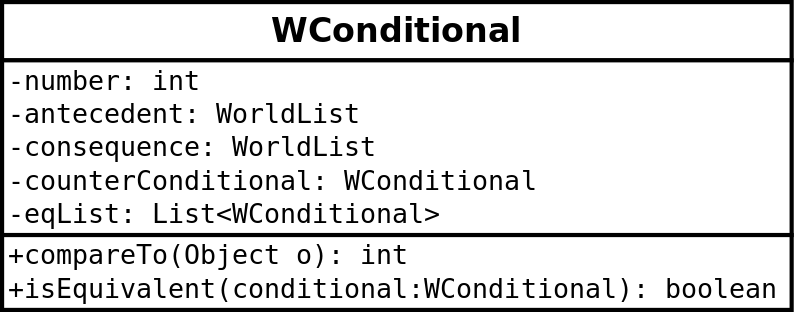
\includegraphics[width=0.55\linewidth]{bilder/wconditional.png}
\caption{WConditional}
\label{pic:wconditional}
\end{figure}

Die Klasse WConditional (W wie worlds) dient dazu, mit zwei der im Abschnitt zuvor beschriebenen WorldsList Objekten Konditionale zu repräsentieren. Der Fokus der Klasse liegt dabei auf der Generierung, Ordnung und Betrachtung von Äquivalenz der Konditionale. Ein vereinfachtes Diagramm der Klasse ist in \autoref{pic:wconditional} zu sehen. Attribute der Klasse sind zum einen Antecedent und Consequence in Form eines WordsList Objekts. Weiterhin die Referenz \textit{counterConditional} ebenfalls als Objekt der Klasse WConditional und einer Liste von äquivalenten Konditionalen als Objekte von WConditional. Außerdem ist die Nummer des Konditionals gemäß der Ordnung $\rdotl$ gemäß Definition \ref{def:sortierung-nfc} als int Variable enthalten.



\begin{figure}
\begin{lstlisting}
public int compareTo(Object o) {
    WConditional otherConditional = (WConditional) o;
    if (this.antecedent.compareTo(otherConditional.getAntecedent()) != 0)
        return this.antecedent.compareTo(otherConditional.getAntecedent());
    else return this.consequence.compareTo(otherConditional.getConsequence());
}
\end{lstlisting}
\caption{Implementierung compareTo(Object o) der Klasse WConditional}
\label{code:compare-wconditonal}
\end{figure}


Die Klasse WConditional ist ebenfalls sortierbar mit dem Interface \textit{Comparable}, die Implementierung der \textit{compareTo(Object 0)} Methode ist in \autoref{code:compare-wconditonal} gezeigt. Die Implementierung entspricht damit genau der Sortierung nach $\overset{\mathrm{c}}{\dotll}$ wie in \autoref{eq:conditional-order} beschrieben.



\begin{figure}
\begin{lstlisting}
public boolean equals(Object o) {
    if (!(o instanceof WConditional))
        return false;
    else {
        WConditional otherConditional = (WConditional) o;
        boolean leftEquals = otherConditional.getConsequence().equals(consequence);
        boolean rightEquals = otherConditional.getAntecedent().equals(antecedent);
        return leftEquals && rightEquals;
    }
}
\end{lstlisting}
\caption{Implementierung \textit{equals(Object 0)} der Klasse WConditonal}
\label{code:equals-wconditonal}
\end{figure}


Eine wichtige Methode der Klasse WConditonal ist die Überschreibung der \textit{equals(Object o)} Methode. Diese ist in \autoref{code:equals-wconditonal} zu sehen. Sie liefert dann true zurück, wenn die zwei WorldsList Objekte beider WConditonals dieselben sind. Zwei Instanzen von WorldsList sind genau dann die selben, wenn sie die selben Welten enthalten. Intern wird hier einfach die Elemente der beiden \textit{List<Integer> worldsList} miteinander verglichen. Die Methode \textit{createEquivalentConditonals(..)} ist in \autoref{sec:counter-conditonals} genauer beschrieben. \\
Nicht zu verwechseln mit der \textit{equals(..)} Methode ist die Methode \textit{isEquivalent(WConditional other)}, diese wird in \autoref{sec:equivalence} beschrieben.
\subsubsection{Berechnung aller Konditionale}


In \autoref{sec:worldslist} wurden bereits die 255 verschiedenen Kombinationen der möglichen Welten unter Signatur $\Sigma_{abc}$ gebildet. In diesem Abschnitt wird gezigt, wie aus diesen Kombinationen alle möglichen Konditionale in Normalform als Objekte der gerade beschriebenen Klasse WConditional generiert werden. \\
Als Input dafür wird die Liste an WorldsLists aus \autoref{sec:worldslist} der ausgewählten Signatur verwendet. Der Algorithmus zur Generierung aller möglichen Kombinationen daraus ist in \autoref{code:create-conditionals} zu sehen. Der Output der Methode ist eine Liste aller möglichen Konditionale in Normalform. \\
Dazu iteriert der Algorithmus in Zeile 4 über alle möglichen Mengen von Welten, diese bilden dann jeweils den Antecedent der Konditionale. Für jede dieser Iterationen werden im Zeile 8 alle echten Teilmengen des Antecedent gebildet, woraus sie die Consequence entsteht. Aus Antecedetnt und Consequence wird dann jeweils ein Konditional gebildet. Zum Schluss werden die Konditionale in Zeile 15 nach der Ordnung $\dotl$ in \autoref{eq:conditional-order} sortiert. Bei Ausführung mit der Signatur $\Sigma_{ab}$ ergeben sich die 50 Konditionale wie in \cite{beierle19} dargestellt. Bei Ausführung mit $\Sigma_{abc}$ entstehen 6050 Kontitionale. Die Anzahl von 6050 Konditionalen für eine Signatur aus drei Elementen entspricht auch der Angabe eben dieser Menge in  der Quelle \cite{beierle19b}. Die Konditionale können in der GUI des Programms NFC Creator mit dem Button CONDITIONALS betrachtet werden.

\begin{figure}
\begin{lstlisting}
private List<WConditional> createBasicConditionalList(List<WorldsList> worldsList) {
    List<WConditional> basicConditionalList = new ArrayList<>();
    for (WorldsList currentWorld : worldsList) {
        List<WConditional> currentConditionalList = new ArrayList<>();
        List<WorldsList> allSubSetsOfCurrentWorld = createSubSetList(currentWorld.getWorldsList());
        for (WorldsList currentSubSworld : allSubSetsOfCurrentWorld) {
            //only add real subsets not the set itself
            if (!currentSubWorld.equals(currentWorld))
                currentConditionalList.add(new WConditional(currentSubWorld, currentWorld));
        }
        basicConditionalList.addAll(currentConditionalList);
    }
    Collections.sort(basicConditionalList);
  return basicConditionalList; }
\end{lstlisting}
\caption{Algorithmus zur Generierung aller Konditionale aus einer gegebenen Liste Möglicher Kombinationen von Welten}
\label{code:create-conditionals}
\end{figure} 


\subsubsection{Äquivalenzklassen und Sortierung der Konditionale}
\label{sec:equivalence}


Im Abschnitt zuvor wurden die Konditionale nach der Ordnung $\dotl$ erstellt. In diesem Abschnitt wird beschrieben wie die Sortierung nach der Ordnung $\rdotl$, welche unter unter \autoref{def:sortierung-nfc} dargestellt wurde, für die Klasse WConditional implementiert ist. Dazu müssen die Konditionale zunächst in Äquivalenzklassen wie in \autoref{sec:äquivalenz-konditionale} gezeigt gruppiert und dann untereinander sortiert weden. \\
Um zu prüfen, ob ein Objekt der Klasse WContitional äquivalent zu einem Anderen ist, besitzt die Klasse die Methode \textit{isEquivalent(WConditonal otherConditional)}, die in \autoref{code:test-equivalence} dargestellt ist. In diesem Algorhitmus wird geprüft, ob sich in der Liste der äquivalenten Konditionale (getBasicEquivalents()) ein äquivalentes Konditional zum übergebenen Konditional (otherConditional) existiert und entsprechend true oder false zurückgegeben. Die Methode \textit{getBasicEquivalents()} gibt eine Liste and WConditional Objekten zurück, mit der Methode \textit{createBasicEquivalents()} erstellt wird. Diese Liste äquivalenter Konditionale beinhaltet dabei jedoch \textit{neu erstellte} Objekte äquivalenter Konditionale, nicht die \textit{tatsächlichen} Objekte der Äquivalenten Konditionale. Die tatsächlichen Objekte können erst nachher gruppiert werden. Ursprünglich sollte die Methode zum testen der Äquivalenz diese Liste der Äquivalenten Konditionale bei jedem Test erstellen, allerdings ist die Generierung sehr Zeitaufwendig und die Äquivalenz wird während der Berechnung der Konditionale sehr oft geprüft (mit $\Sigma_{ab}$ 1550 mal, mit $\Sigma_{abc}$  16.784.250 mal), sodass die Methode \textit{getBasicEquivalents()} sicherstellt, dass die Liste Äquivalenter Konditionale nur einmal erzeugt wird. Die Zeiteinsparung dadurch ist deutlich spürbar.\\ 
Die Methode zur Erstellung der Liste der äquivalenten Konditionale ist in \autoref{code:create-equivalents} abgebildet. In Zeile 3 und 4 wird für Antecedent und Consequence jeweils eine Liste der Umbenennungen erstellt wie in \autoref{sec:worldslist} bereits gezeigt wurde. Über diese Umbenennungen wird in Zeile 6 iteriert und für alle Paare von Antecedent und Consequence wird ein neues Konditional als mögliche Umbenennung gespeichert, wenn die Umbenennung wirklich verschieden vom Ausgangskonditional ist. Wenn ein Konditional keine äquivalenten Konditionale besitzt, sind die Umbenennungen an dieser Stelle sonst gleich wie das Ursprungskonditional. Beispielsweise würden Umbenennungen des Konditionals $(ab|!a!b,ab)$ sonst immer wieder das gleiche Konditional entstehen lassen.


\begin{figure}
\begin{lstlisting}
public boolean isEquivalent(WConditional otherConditional) {
    for (WConditional eqConditional : getBasicEqList())
        if (otherConditional.equals(eqConditional))
            return true;
    return false;
}
\end{lstlisting}
\caption{Algorithmus zur Prüfung der Äquivalenz der Klasse WConditional}
\label{code:test-equivalence}
\end{figure} 


Der Ablauf der Erstellung der Liste der Konditionale NFC ist dann wie folgt: Der NFC Creator beginnt dann durch die Liste der Konditionale zu iterieren und erstellt für jedes gefundene Konditional eine eigene Liste. Für jedes dieser Konditionale wird dann mit der \textit{isEquivalent(..)} Methode der Rest der urprünglichen Liste auf Äquivalenz überprüft und die \textit{tatsächlichen} Objekte der äquivalenten Konditionale werden in die Liste eingefügt und aus der ursprünglichen Liste entfernt. Die neue Liste wird dann jeweils mit der \textit{compare(..)} Methode sortiert. Dadurch entsteht eine Liste von Listen von den tatsächlichen Objekten der äquivalenten Konditionale. Diese Darstellung enspricht dann der Darstellung der Konditionale in \cite{beierle19}. Mit dem NFC Viewer kann diese Ansicht mit dem Botton CNFCEQ erstellt werden. Die Menge der kanonischen Konditionale $(cNFC)$ ergibt sich daraus als eine Liste der jeweils ersten Elemente der Listen der äquivalenten Konditionale. Diese kann im NFC Viewer mit dem Button CNFC angezeigt werden.
Die mit CNFCEQ erstelle Darstellung kann nun genutzt werden, um die Konditionale sortiert nach $\rdotl$ in eine neue Liste NFC aufzunehmen. Dazu wird eine neue Liste von WConditonal erstellt. Zunächst werden alle Listen mit äquivalenten Konditionalen iteriert, welche in sich nach $\dotl$ sortiert sind. Von diesen Listen wird jeweils das erste Element in die neue Liste NFC eingefügt. Dann werden die Listen erneut iteriert und alle Elemente außer dem ersten in die Liste NFC eingefügt. Als Ergebis entsteht die List<WConditional> NFC die genau der Sortierung $\rdotl$ entspricht. Betrachtet werden kann die Liste NFC mit dem Button NFC im NFC Viewer. Man beachte, der NFC Viewer erstellt mit den Buttons CONDITIONALS und NFC die selbe Menge an Konditionalen, nur sind die CONDITIONALS nach $\dotl$ und NFC nach $\rdotl$ sortiert. \\
Für die Signatur $\Sigma_{abc}$ ergeben sich wie schon beschrieben insgesamt 6050 Konditionale. Diese Menge beinhaltet 2774 Äquivalenzklassen und demzufolge hat auch die Menge der kanonischen Konditionale $cNFC$ 2774 Konditionale.


\begin{figure}
\begin{lstlisting}
private void createBasicEquivalents() {
    basicEqList = new ArrayList<>();
    List<WorldsList> antecedentList = antecedent.createRenamings();
    List<WorldsList> consequenceList = consequence.createRenamings();
    for (int i = 0; i < antecedentList.size(); i++) {
        WConditional possibleEqConditional = new WConditional(consequenceList.get(i), antecedentList.get(i));
        //dont add the conditional to itselfs eq conditionals
        if (!this.equals(possibleEqConditional))
            basicEqList.add(possibleEqConditional);
    }
}
\end{lstlisting}
\caption{Algorithmus zur Generierung einer Liste der äquivalenten Konditionale der Klasse WConditional}
\label{code:create-equivalents}
\end{figure} 




\subsubsection{Counter Conditionals}
\label{sec:counter-conditonals}
Für den Algorithmus GenKB ist es nötig, dass zu einem Konditional schnell dass CounterConditional zur Verfügung steht. Mit der Klasse WConditional wird das vorbereitet. Analog zum Finden der äquivalenten Konditionale besitzt dazu jedes Konditional zum Einen eine Methode, um zunächst ein \textit{neues} CounterConditional zu erstellen. Wenn dann alle Konditionale erstellt sind, wird nach dem \textit{tatsächlichen} Objekt des CounterConditional gesucht und eine Referenz dazu im ursprünglichen Konditional gesetzt. \\
Um das vorläufige CounterConditional zu generieren wird in der Methode \textit{getBasicCounterConditional()} zunächst ein \textit{neues} Konditional generiert, wie in \autoref{code:basic-counter} dargestellt. Als Antecedent für das neue Konditonal wird das Antecedent des alten verwendet, dieses bleibt ja gleich. Als Consequence wird die Liste der Welten des Antecedent minus der Liste der Welten der Consequence des ursprünglichen Konditionals gebildet. Die Methode \textit{getBasicCounterConditional()} wird dann später verwendet, um mit der Methode \textit{findCounterConditional(...)} aus \autoref{code:real-counter} über NFC zu iterieren und damit dann das tatsächliche CounterConditonal zu setzen. Im Programm NFC Viewer kann mit dem Button NFC$\_$COUNTER die Menge NFC mit den dazugehörigen Counter Konditionale angezeigt werden.

\begin{figure}
\begin{lstlisting}
public WConditional getBasicCounterConditional() {
    WorldsList newConsequence = new WorldsList();
    newConsequence.addList(antecedent.getWorldsList());
    newConsequence.removeWorlds(consequence);
    return new WConditional(newConsequence, antecedent);
}
\end{lstlisting}
\caption{Algorithmus zur Generierung des vorläufigen Counter Conditionals der Klasse WConditional}
\label{code:basic-counter}
\end{figure} 


\begin{figure}
\begin{lstlisting}
private WConditional findCounterConditional(WConditional conditional, List<WConditional> nfc) {
    for (WConditional possibleCounterConditional : nfc)
        if (conditional.getBasicCounterConditional().equals(possibleCounterConditional))
            return possibleCounterConditional;
    return null;
}
\end{lstlisting}
\caption{Algorithmus zur Generierung des tatsächlichen Counter Conditionals der Klasse NFC Creator}
\label{code:real-counter}
\end{figure} 



\subsection{Grafische Oberfläche zum Betrachten der Konditionale}


Der NfcCreator hat eine kleine grafische Oberfläche namens \textit{NfcViewer}, ein Screenshot davon ist in \autoref{pic:nfc-viewer} zu sehen. Damit können die erstellten Konditionale betrachtet und auch als Textdatei gespeichert werden. Es ist so auch möglich, Teilergebnisse aus dem Erstellungsprozess der Konditionale anzuzeigen, um den Vorgang besser nachvollziehen zu können.


\begin{figure}
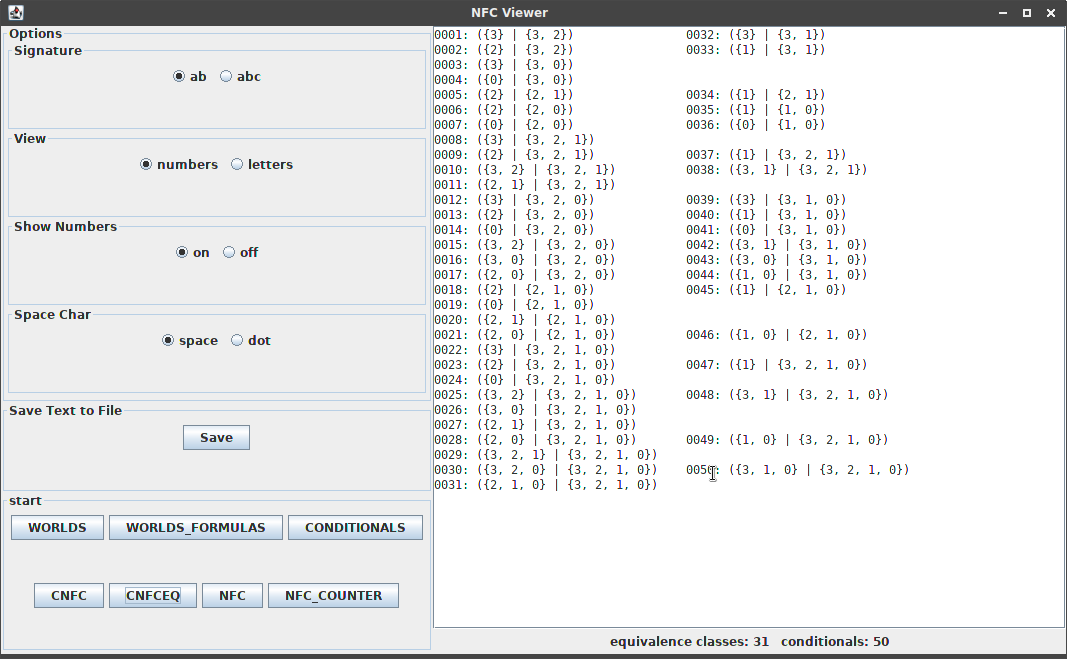
\includegraphics[width=0.9\linewidth]{bilder/nfc-viewer.png}

\caption{Screenshot NFC Viewer mit Ansicht analog zu Tabelle 1 aus \cite{beierle19}}
\label{pic:nfc-viewer}
\end{figure}



Der grundsätzliche Aufbau der GUI des NfcViewers besteht aus zwei Teilen. Links befinden sich im oberen Bereich die Optionen, darunter befinden sich die Buttons mit den möglichen Aktionen. Auf der rechten Seite ist ein Textfenster, welches das Ergebnis der gewählten Optionen und Aktion zeigt. Unter dem Textfeld steht jeweils eine kurze Beschreibung des Inhalts des Textfeldes. \\
Im Folgenden werden die Optionen im Menü erklärt. Die Auswahl der Signature bietet selbsterklärend die Möglichkeiten $ab$ und $abc$. Die Option \textit{View} stellt ein, ob eine mögliche Welt in Buchstabenform oder als Repräsentation als Zahl analog der Darstellung in \cite{beierle19} erfolgen soll. Beispielsweise wird so mit Signatur$\Sigma_{ab}$ die mögliche Welt $a \overline{b}$ entweder als $a!b$ oder als 2 dargestellt. Mit der Option \textit{ShowNumbers} lässt sich einstellen, ob die angezeigten Objekte, beispielsweise Konditionale, nummeriert dargestellt werden sollen oder nicht. Die letzte Option \textit{SpaceChar} stellt einen Platzhalter für mehrere auf einer Zeile angezeigte Objekte ein. Im Screenshot ist die Option auf Space gesetzt. Wird Dot aktiviert, werden zeilenweise kleine Punkte angezeigt, damit der Betrachter die Zeilen am Bildschirm etwas leichter verfolgen kann als auf rein weißem Untergrund. Das untenliegende Feld bietet mit dem Save Button die Möglichkeit, den Inhalt des Textfensters zu speichern.



\subsection{Modellierung der Konditionale mit Aussagenlogik}
Nachdem die Menge der Konditionale nun berechnet und sortiert ist, sollen daraus konsistente Wissensbasen generiert werden. Dazu sind die Konditionale in ihrer bisherigen Form als Instanzen von WConditional allerdings ungeeignet. Deshalb werden sie in Objekte der neuen Klasse PConditonal (P wie propositional logic) umgewandelt. Mit diesen ist dann die Verarbeitung von Aussagenlogik möglich und somit auch die Generierung der Wissensbasen. Im Folgenden wird der Weg dahin beschrieben.




\subsubsection{Implementierung der Aussagenlogik}
\label{sec:logic}

Um bei der Generierung von Wissensbasen Aussagenlogik verwenden zu können, ist ein kleines Framework nötig welches die benötigten Elemente der Aussagenlogik als Java Objekte abbildet und somit die üblichen Operationen mit diesen ermöglicht. Die Idee die Logik so abzubilden wie im Folgenden beschrieben stammt aus dem Framework zu InfOCF, die konkreten Implementierungen sind jedoch verschieden. Im Folgenden werden die später verwendeten Elemente der Aussagenlogik als Java Implementierung kurz vorgestellt.



\paragraph{World und Signature}
Variablen zur Bezeichnung einzelner Atome werden mit der Enum \textit{Var} dargetellt, welche die Werte $a$, $b$ oder $c$ annehmen kann. Die Basis für die möglichen Welten bildet dann Klasse \textit{AbstractWorld}. Diese bietet die abstrakte Methode \textit{boolean get(Var var)}. Implementiert wird die Klasse \textit{AbstractWorld} von den konkreten Klassen \textit{ABWorld} und  \textit{ABCWorld}. Diese beiden konkreten Klassen repräsentieren jeweils eine mögliche Welt mit zwei oder drei vorhandenen Variablen. Für jede der enthaltenen Variablen existiert in der \textit{AbstractWorld} Implementierung ein boolean Wert der true oder false sein kann. Die Welten bieten \textit{toString()} Methoden und Getter für die boolean Variablen. \\
Die Signatur wird mit der abstrakten Basisklasse  \textit{AbstractSignature} und den konkreten Klassen \textit{AB} und  \textit{ABC} abgebildet. Die Implementierungen von AbstractSignature erfüllen im wesentlichen zwei Funktionen: Zum Einen dienen sie als Indikator, welche Signatur gewählt wurde. Zum Anderen besitzen sie jeweils eine List<AbstractWorld>,  die alle möglichen Welten als Instanz von AbstractWorld der gewählten Signatur beinhaltet. Die Liste der möglichen Welten kann so für diverse Operationen der Aussagenlogik abgerufen werden. Benötigt werden diese Listen der möglichen Welten insbesondere zur Evaluation und zum Vergleich von aussagenlogischen Termen.

\paragraph{AbstractFormula}


\begin{figure}
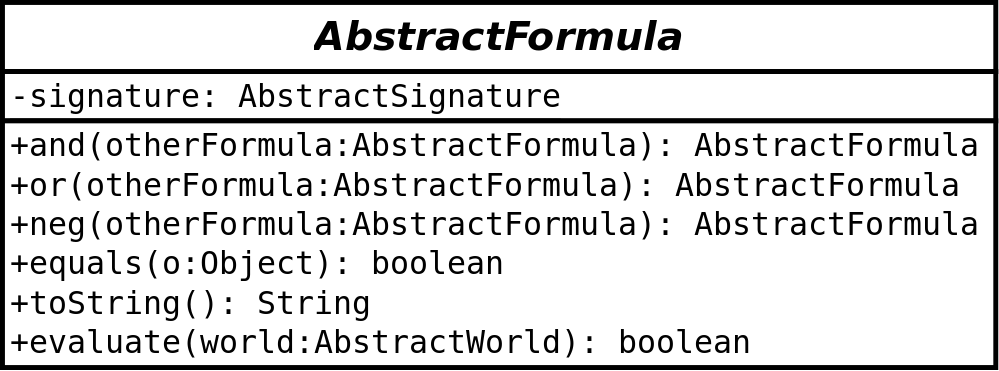
\includegraphics[width=0.55\linewidth]{bilder/AbstractFormula.png}
\caption{Klassendiagramm AbstractFormula}
\label{pic:abstractformula}
\end{figure}


Die grundlegende Klasse der Aussagenlogik ist die abstrakte Klasse AbstractFormula, welche in \autoref{pic:abstractformula} als Klassendiagramm dargestellt wird. Alle Aussagen basieren auf dieser Klasse und entsprechend erben alle Aussagen repräsentierenden Objekte von dieser. Sie stellt die so Schnittstelle für alle Aussagen dar und bietet auch selbst einige Funktionen. Die einzige Variable ist die gewählte Signatur \textit{signature} in Form einer Instanz von AbstractSignature als statisches Objekt für alle Instanzen von erbenden Objekten. Weiterhin besitzt die Klasse 6 Methoden, von denen 4 konkret implementiert und 2 abstrakt sind. Implementiert ist zum einen die Methode \textit{and(AbstractFormula otherFormula)}, sie gibt einfach ein Objekt \textit{Conjunction} zurück welches eine Konjunktion aus dem aktuellen (this) Objekt und dem übergebenen ist. Überschrieben wird diese Methode nur in der Klasse Conjunction. Analog dazu verhält sich die Methode \textit{or(AbstractFormula otherFormua)}, welche ein Object der Klasse \textit{Disjunction} zurückgibt. Diese Methode wird ausschließlich von der Klasse \textit{Disjunction} überschrieben. Die dritte konkret Implementierte Methode ist die Negation, aufrufbar mit \textit{neg()} ohne Parameter. Diese Methode gibt eine Negation in Form von \textit{new Negation(this)} zurück. Überschrieben wird diese Methode nur im der Klasse \textit{Negation} selbst. Die letzte konkrete Methode der Klasse \textit{AbstractFormula} ist die Methode \textit{equals(Object o)}, die in \autoref{code:equals-formula} gezeigt ist. Sie ist als \textit{final} deklariert und wird demzufolge von keiner erbenden Klasse überschrieben. Wie im Code zu sehen, überprüft die Methode zuerst, ob das übergebene Objekt eine Instanz der Klasse \textit{AbstractFormula} darstellt. Dann wird für alle möglichen Welten der Signatur geprüft, ob die Evaluierung der Welt des übergebenen Objekts das gleiche Ergebnis zurückgibt wie die Evaluierung des aktuellen Objekts (this). Ist das einmal nicht der Fall, wird sofort false zurückgegeben. Wenn die Evaluierung für alle möglichen Welten das gleiche Ergebnis zurückgibt, sind die beiden Objekte gleich im Sinne der \textit{equals(..)} Methode. \\
Weiterhin existieren die abstrakten Methoden \textit{evaluate(World world)} und \textit{toString()}, die jeweils von allen erbenden Klassen überschrieben werden.


\begin{figure}
\begin{lstlisting}
public final boolean equals(Object o) {
    if (!(o instanceof AbstractFormula))
        return false;
    for (AbstractWorld world : signature.getPossibleWorlds()) {
        if (!this.evaluate(world) == ((AbstractFormula) o).evaluate(world))
            return false;
    }
    return true;
}
\end{lstlisting}
\caption{\textit{equals(Object o)} Methode der Klasse AbsractFormula}
\label{code:equals-formula}
\end{figure} 



\paragraph{Atom}


Die Klasse Atom repräsentiert einfach ein einzelnes Atom als Aussage und erbt von AbstractFormula. Ein Objekt dieser Klasse besitzt eine Instanzvariable mit dem Namen \textit{variable} des Typs \textit{Var}, die den Wert $a$, $b$ oder $c$ annehmen kann. Die \textit{evaluate(AbstractWorld world)} Methode funktioniert folgendermaßen: Sie schaut auf den Variablennamen der in \textit{variable} gespeichert ist und vergleicht diesen mit dem Wert dieser Variable in der übergebenen AbstractWorld und gibt dann zurück ob die Variable in der AbstractWorld true oder false ist. Die zweite Methode der Klasse Atom überschreibt die \textit{toString()} Methode und gibt einfach den Namen der \textit{variable} als String zurück. Die \textit{toString()} Methoden von komplexeren Aussagen als Atom setzten sich dann aus deren Teilaussagen zusammen und rufen so letztendlich auch die \textit{toString()} Methode der Klasse Atom auf.


\paragraph{Conjunction}


Die Klasse \textit{Conjunction} repräsentiert eine Konjunktion aus einer Menge von AbstractFormulas. Diese werden in einer \textit{ArrayList<AbstractFormula>} gespeichert. Instanzen der Klasse können auf zwei mögliche Arten gebildet werden: Entweder direkt per Konstruktor in Form von \textit{new Conjunction(AbstractFormula...formulas)} oder indem auf einer Instanz von AbstractFormula die Methode \textit{and(AbstractFormula formula)} aufgerufen wird. Dabei ist die Klasse \textit{Conjunction} die einzige AsbstractFormula Implementierung, welche die \textit{and(..)} Methode überschreibt. Sie erstellt im Gegensatz zu allen Anderen eine neue Conjunction mit einer Liste die aus der FormulaList der aktuellen (\textit{this}) Conjunction und der hinzugefügten Conjunction besteht. Dadurch stehen alle Elemente der bisherigen \textit{Conjunction} und der hinzugefügten AbstractFormula gleichberechtigt nebeneinander in der \textit{List<AbstractFormula>}. Ohne diese Überschreibung würde eine \textit{Conjunction} mit einer \textit{Conjunction} als Element entstehen, was zwar korrekt, aber unnötig verschachtelt und in der Darstellung schwerer zu lesen wäre. Bildlich gesprochen werden so einfach die unnötigen Klammern des Terms aufgelöst. Die \textit{toString()} Methode reiht einfach die Elemente der \textit{List<AbstractFormula>} ohne spezielles Zeichen dazwischen zur Verbindung aneinander, entspricht so der verkürzenden Darstellung aus \cite{beierle19}. Die \textit{evaluate(AbstractWorld world)} Methode der Klasse Conjunction evaluiert die einzelnen Teilaussagen aus der FormulaList und gibt falsch zurück sobald ein Element der \textit{List<AbstractFormula>} falsch ist. Das entspricht einer \textit{lazy evaluation} und spart unnötige Rechenoperationen. Erst wenn alle Elemente der \textit{List<AbstractFormula>} true zurückgeben gibt auch die \textit{Conjunction} insgesamt true zurück.


\paragraph{Disjunction}
todo \\

Die Klasse \textit{Disjunction} repräsentiert eine Disjunktion und ist analog zur gerade beschriebenen Klasse Conjunction aufgebaut. Sie beinhaltet eine \textit{ArrayList<AbstractFormula>} in der die Elemente der Konjuntion gespeichert sind. Ebenfalls ist sie per Konstruktor als \textit{new Conjunction(AbstractFormula...formulas)}  mit einem Array instanziierbar. Die Methode der Klasse AbstractFormula \textit{or(AbstractFormula formula)} wird als einzige durch die Klasse \textit{Disjunction} überschrieben und erstellt hier eine neue Conjunction mit einer Liste aus den Elementen der ursprünglichen Conjunction und dem hinzugefügten Element anstatt einer verschachtelten Conjunction. Die \textit{toString()} Methode der Klasse Conjunction gibt die Elemente als String mit einem Komma getrennt aus. Die dritte Methode der Klasse \textit{Disjunction} überschreibt die \textit{evaluate(World world)} Methode der Klasse AbstractFormula. Hier findet ebenfalls eine lazy evaluation statt: Die Methode gibt true zurück sobald ein Teilausdruck der formulaList true ist und gibt false zurück wenn alle Teilausdrücke false zurückgeben.


\paragraph{Negation}


Negation ist die letzte hier beschriebene Implementierung von AbstractFormula. Das einzige Attribut der Klasse ist eine \textit{AbstractFormula} formula, also der Term der negiert wird. Die Klasse ist eine Art Wrapper für die beinhaltete \textit{AbstractFormula}. Ein Objekt kann wieder zum einen direkt per Konstruktor als \textit{new Negation(AbstractFormula formula)} erzeugt werden. Die andere Variante ist das aufrufen der \textit{neg()} Methode auf einer Instanz von \textit{AsbstractFormula}. Die \textit{neg()} Methode der Klasse \textit{AsbstractFormula} wird hier überschrieben und gibt die AbstractFormula zurück. Das Vermeidet das Erstellen einer Negation von einer Negation eines Terms, was zwar korrekt aber unnötig kompliziert wäre. Die \textit{toString()} Methode gibt die eingeschlossene \textit{AbstractFormula} mit vorangestelltem \glqq !\grqq \space  wieder. Falls die \textit{AbstractFormula} dabei keine Instanz von Atom ist wird die \textit{AbstractFromula} dabei von Klammern eingeschlossen, um sie eindeutig interpretierbar zu machen. Die \textit{evaluate} Methode gibt einfach die Umkehrung (Java: \glqq !\grqq) der eingeschlossenen \textit{AbstractFormula} wieder.


\subsubsection{Die Klasse PConditional}
\label{sec:pconditional}
\begin{figure}
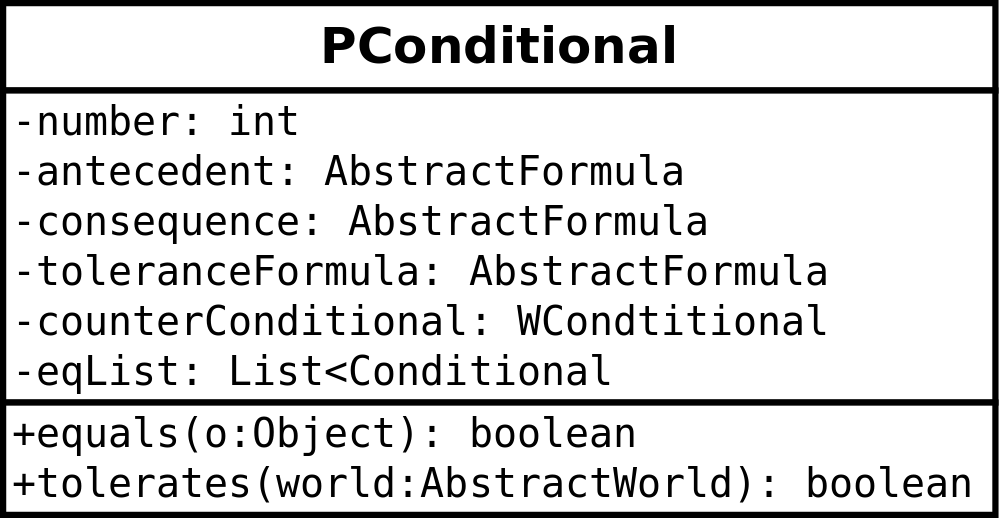
\includegraphics[width=0.55\linewidth]{bilder/PConditional.png}
\caption{PConditional}
\label{pic:pconditional}
\end{figure}


Die Klasse PConditional repräsentiert ein Konditional und unterstützt im Gegensatz zur Klasse WConditional die Verarbeitung mit Aussagenlogik. Ein vereinfachtes Klassendiagramm von PConditional ist in \autoref{pic:pconditional} zu sehen. Die meisten Attribute werden bei der Übersetzung von WConditional zu PConditional übernommen. Wie genau diese Übersetzung abläuft, ist in \autoref{sec:übersetzung} beschrieben. Als Attribute besitzt die Klasse neben der Nummer des Konditionals ein Antecedent und Consequence jeweils in Form einer AbstractFormula. Dazu kommt eine Referenz zu einem Konditional \textit{coutnerConditional} und eine Liste der äquivalenten Konditionale.


\begin{figure}
\begin{lstlisting}
public boolean isToleratedBy(List<PConditional> conditionalList) {
    for (AbstractWorld world : signature.getPossibleWorlds()) {
        if (this.shortAntecedent.evaluate(world) && this.shortConsequence.evaluate(world)) {
            boolean toleratesAll = true;
            for (PConditional conditional : conditionalList) {
                if (!conditional.tolerates(world)) {
                    toleratesAll = false;
                    break;
                }
            }
            if (toleratesAll)
                return true;
        }
    }
    return false;
}
\end{lstlisting}
\caption{\textit{isToleratedBy(List<PConditional> conditionalList)} Methode der Klasse PConditional}
\label{code:conditional-istoleratedby}
\end{figure}



Die wichtige Methode \textit{isToleratedBy(List<PConditonal> list)} der Klasse PConditional ist in \autoref{code:conditional-istoleratedby} gezeigt. Mit dieser Methode wird geprüft, ob ein Konditional von einer Liste von Konditionalen (einer Wissensbasis) toleriert wird. Das ist somit die praktische Umsetzung der Toleranz wie sie unter \autoref{def:toleranz} bereits beschrieben wurde. Dieser Test wird benötigt, um die Konsistenz einer Wissensbasis zu überprüfen. Sie funktioniert folgenermaßen: In Zeile 2 wird über alle möglichen Welten iteriert. Wenn in Zeile 3 die Bestätigung des aktuellen Konditionals durch die Welt festgestellt wird, wird in den folgenden Zeilen geprüft, ob alle Konditionale der Liste die mögliche Welt tolerieren. Ist das der Fall, wird in Zeile 12 true zurück gegeben. Wenn nicht, wird der Ablauf für die verbleibenden Welten wiederholt. Wenn das Konditional für keine mögliche Welt von der Liste toleriert wird, wird in Zeile 15 false zurück gegeben. \\
Die \textit{equals(Object o)} Methode der Klasse PCodnitional ist der Einfachheit halber so implementiert, dass sie true zurückgibt, wenn das übergebene Objekt ein PConditional mit derselben Nummer ist. Das ist wesentlich schneller als jeweils \textit{equals()} von Antecedent und Consequence zu überprüfen. Das Ergebnis ist aber in diesem Fall das selbe, da nur eine fest definierte und nummerierte Menge von Konditionalen verwendet wird.


\subsubsection{Übersetzung der Konditionale}
\label{sec:übersetzung}
In diesem Abschnitt wird beschrieben, wie die Konditionale aus der Form als Instanzen von WConditional in Instanzen von PConditional übertragen werden. Genauer gesagt ist der interessante Teil, wie Antecedent und Consequence jeweils aus der Form WorldsList in die Form AbstractFormula gebracht werden. \\
Dabei sind zwei grundsätzliche Vorgehensweisen vorstellbar: Der naheliegende Ansatz ist der folgende: Die Liste der möglichen Welten wird als Disjunktion von Konjunktionen aufgefasst. Als Beispiel, unter Signatur $\Sigma_{ab}$ sei Liste Möglicher Welten $ab, !ab$ gegeben. Dann ist der aussagenlogische Term dafür $(a \wedge b) \vee (\overline{a}\wedge b)$. Diese Formel ist recht umständlich, aber korrekt. Mit Signatur $\Sigma_{abc}$  werden die Formeln sogar noch länger, die Längste ist dann eine Disjunktion aus 8 Konjunktionen. Ein großer Vorteil an dem Ansatz ist zum einen, dass die Normalform von NFC verwendet wird und somit eine Systematik herrscht. Der andere Vorteil ist, dass diese Übersetzung so einfach für alle Konditionale nach dem gleichen System erfolgen kann. Dieser Variante wurde nach einigem Testen der Vorzug gegeben.\\
Der andere Ansatz wäre es, eine möglichst kurze Formel für den Term aus Normalform zu finden. So könnte man beispielsweise im gerade beschriebenen Beispiel auch die Formel $a$ verwenden. Vorteil wären hier in vielen Fällen weniger umständliche Formeln und die Hoffnung, dass der Programmablauf möglicherweise durch einfache Formeln beschleunigt werden kann. Nachteile sind, dass es schwer ist, die kürzeste Formel für jeden Fall zu finden und dass die Einheitlichkeit verloren geht, besonders, wenn nicht immer die kürzeste Formel gefunden wird. Aufgrund dieser Nachteile wurde diese Variante nach einigem Testen wieder verworfen, was in diesem Abschnitt später noch etwas genauer dargestellt wird.\\
Unabhängig von der genauen Übersetzung der Formeln für Antecedent und Consequence läuft die Übersetzung der Konditionale wie folgt ab: Es wird für jedes WConditional ein PConditional erstellt, für welches Antecedent, Consequence, Number, CounterConditional und die Liste der äquivalenten Konditionale übertragen werden. Das ganze findet im Programm im Teil \textit{NnfCreator} statt. \\
Nun zum Vergleich der Varianten für die Übersetzung von Antecedent und Consquence: Beide  Versionen der Übersetzung der Konditionale können von der Klasse \textit{ConditionalTranslator} vorgenommen werden. Die erste Variante, die Übersetzung in Normalform, ist recht einfach: Es wird einfach jeweils für Antecedent und Consequence die WorldsList als Disjunktion von Konjunktionen zusammengesetzt. Die zweite Variante ist schwerer Umzusetzen. Um zu testen, ob sie einen relevanten Geschwindigkeitsvorteil bieten kann, wurde für etwa die Hälfte der mit $\Sigma_{abc}$ 255 möglichen Formeln eine kürzere Variante gefunden, die Übersetzungen befinden sich im Unterordner \textit{resources} als Textdateien. Der ConditionalTranslator verwendet dann wenn möglich für den Test die kürzere Variante. Zur Sicherheit wird die kürzere Variante auch auf Äquivalenz mit der Variante in Normalform geprüft, um Übersetzungsfehler auszuschließen. \\
Diese beiden Varianten wurden nun in Bezug auf Geschwindigkeit verglichen. Als Test wurde die Zeit der Iteration von GenkB für $k=1$ mit $\Sigma_{abc}$ gemessen und mehrere Testdurchläufe in beiden Varianten getestet. Als Ergebnis hat sich die Variante mit den kurzen Formeln 10-15 $\%$ schneller als die Variante in Normalform erwiesen. Der Geschwindigkeitsvorteil war somit geringer als erhofft und in Anbetracht der Nachteile wurde diese Variante wieder verworfen. Die Möglichkeit der kürzeren Übersetzungen ist aber mit der Klasse ConditionalTranslator weiterhin im Code vorhanden und könnte bei Bedarf verbessert und einfach wieder eingebaut werden. \\
Ein anderer Versuch, um die Vorteile beider Varianten zu kombinieren, wurde nach kurzem Testen wieder Verworfen. Dazu sollten die Klassen PConditional jeweils zwei Formeln für Antecedent und Consequence enthalten. Einmal die Normalform, um diese ausgeben zu können und einmal die kurze Form, um den Vorteil der etwas höheren Rechengeschwindigkeit nutzen zu können. Das Ergebnis war allerdings, dass mit dieser komplizierten Variante überraschenderweise nur die Geschwindigkeit in Normalform erreicht werden konnte. Die kurzen Formeln konnten nicht mehr zu einer höheren Geschwindigkeit beitragen. Der Grund dafür ist nicht genau geklärt, aber es bestehe eine Vermutung: In dieser Variante besitzt jede PConditional Instanz 4 anstatt 2 Objekte des Typs AbstractFormula als Instanzvariablen, wodurch die Objekte jeweils wesentlich mehr Speicher benötigen dürften. Dadurch müssen während des Programmablaufs wesentlich mehr Daten zwischen Prozessor und Hauptspeicher hin und her geladen werden. Dieser zusätzliche Speicherverbrauch könnte die mangelnde Geschwindigkeit möglicherweise erklären. Da diese Variante also keine Vorteile bietet wurde sie wieder komplett verworfen und aus dem Code entfernt.


\subsubsection{Wissensbasen}



\begin{figure}
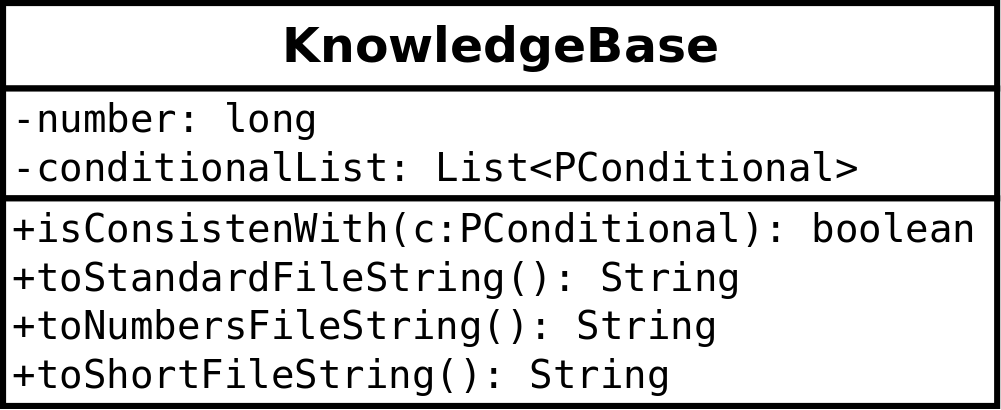
\includegraphics[width=0.45\linewidth]{bilder/KnowledgeBase.png}
\caption{Klassendiagramm KnowledgeBase}
\label{pic:knowledgebase}
\end{figure}



Wissensbasen werden durch Objekte der Klasse KnowledgeBase repräsentiert. Ein vereinfachtes Klassendiagramm ist in \autoref{pic:knowledgebase} zu sehen. Als Instanzvariablen besitzt die Klasse die Nummer der Wissensbasis als long Wert und eine Liste der in der Wissensbasis enthaltenen Konditionale in Form einer \textit{ArrayList<PConditional>}. Die Nummer der Wissensbasis wird immer gleich im Konstruktor von der GenKB Implementierung gesetzt und ist als eine \textit{final} Refererenz implementiert, damit sie nachträglich nicht mehr geändert werden kann.\\
Eine wichtige Methode der Klasse ist \textit{isConsistentWith(PConditional c)}. Mit dieser wird geprüft, ob die vorhandene Wissensbasis mit dem als Parameter übergebenem Konditional eine neue konsistente Wissensbasis ergeben würde. Der Aufruf dieser Methode entspricht damit der Zeile 10 von GenKB. Die konkrete Implementierung dieser Methode ist in \autoref{code:kb-consistent} abgebildet. Dieser Algorithmus ist die Umsetzung des bereits in \autoref{sec:wissensbasen} dargestellten Tests auf Konsistenz für Wissensbasen.  Die Idee zu dieser Implementierung stammt auch aus der Umsetzung des Tests auf Konsistenz von Wissensbasen aus InfOCF, ist hier jedoch etwas verkürzt. Denn in der hier vorgestellten Implementierung wird keine geordnete Partitionierung der Wissensbasis erstellt, da diese nicht benötigt wird. Das sollte die Methode etwas beschleunigen. Der Rückgabewert als boolean zeigt an, ob die betroffene Wissensbasis, auf dessen Objekt die Methode aufgerufen wird, mit dem übergebenen Konditional eine konsistente Wissensbasis ergeben würde oder nicht.


\begin{figure}
\begin{lstlisting}
public boolean isConsistentWith(PConditional conditionalToTest) {
    List<PConditional> listToTest = new ArrayList<>(this.conditionalList);
    listToTest.add(conditionalToTest);
    while (!listToTest.isEmpty()) {
        List<PConditional> listToRemove = new ArrayList<>();
        for (PConditional conditional : listToTest) {
            if (conditional.isToleratedBy(listToTest)) {
                listToRemove.add(conditional);
            }
        }
        if (listToRemove.isEmpty())
            return false;
        listToTest.removeAll(listToRemove);
    }
    return true;
}
\end{lstlisting}
\caption{\textit{isConsistentWith(PConditional p)} Methode der Klasse PConditonal}
\label{code:kb-consistent}
\end{figure} 
todo: list to test leer? 2 mal genannt? \\

Die Methode zum Testen auf Konsistenz aus \autoref{code:kb-consistent} funktioniert folgendermaßen: Aufgerufen wird sie auf einer KnowledgeBase, als Parameter wird ein Konditional übergeben. Ziel ist es herauszufinden, ob die Wissensbasis mit dem übergebenen Konditional eine neue konsistente Wissensbasis ergeben würde. Dazu wird zunächst in den Zeilen 2 und 3 eine Liste \textit{listToTest} mit den Konditionalen der Wissensbasis und dem zusätzlich übergebenem Konditional erstellt. Danach wird in Zeile 4 eine while Schleife ausgeführt, solange die gerade erzeugte List nicht leer ist. Darin werden in jedem Durchlauf alle Konditionale von der Liste in eine neue Liste verschoben, welche von \textit{listToTest} toleriert werden. Wenn diese neue Liste leer ist, ist \textit{listToTest} inkonsistent und es wird false zurückgegeben. Ansonsten wird die neue Liste von \textit{listToTest} entfernt und ein neuer Durchlauf der while Schleife beginnt. Wenn \textit{listToTest} leer ist, wird true zurück gegeben. \\
Daneben besitzt die Klasse KnowledgeBase neben der "normalen" noch drei \textit{toString()} Methoden. Die erste ist die \textit{toStandardFileString()} Methode, die aus der Wissensbasis in einen InfOCF kompatiblen String erzeugt, um in in eine Datei zu schreiben. Weiterhin exisitiert eine \textit{toNumbersFileString()} Methode, welche die Wissensbasis in einen Text umwandelt bei dem die Konditionale als Nummer dargestellt werden. Als dritte Variante steht eine \textit{toShortFileString()} Methode zur Verfügung. Damit wird eine besonders kurze Repräsentation der Wissensbasis erzeugt, die beim Schreiben von Pairs auf die Festplatte genutzt wird, wie es unter \autoref{sec:realpair} gezeigt wird. \\
Für die Klasse KnowledgeBase existieren drei Konstruktoren: Der einfachste \textit{KnowledgeBase(long number, PConditional conditional)} wird für die Initialisierung der Wissensbasen mit jeweils einem Element in Zeile 5 von GenKb verwendet. In allen anderen Iterationen wird der Konstruktor \textit{KnowledgeBase(long number, KnowledgeBase knowledgeBase, PConditional conditionalToAdd)} für die Mehrelementigen Wissensbasen in Zeile 12 GenKB benutzt. Die dritte Variante in der Form \textit{KnowledgeBase(String stringFromFile)} kommt zum Zug, wenn die Wissensbasen aus Textdateien von der Festplatte rekonstruiert werden sollen wie in \autoref{sec:hddBuffer} beschrieben. \\
Ursprünglich existierte auch eine Implementierung einer Wissensbasis, die anstatt einer List<WConditional> eine List<Integer> zur Repräsentation der Konditionale verwendet hat. Dies sollte Arbeitsspeicher sparen. Die Ersparnis war aber gering, dafür kostete das Verfahren recht viel Rechenzeit, daher wird dieses Verfahren nicht mehr genutzt.



\section{Berechnung der Wissensbasen}
\label{sec:kbcreator} % ref used by overview



\begin{figure}
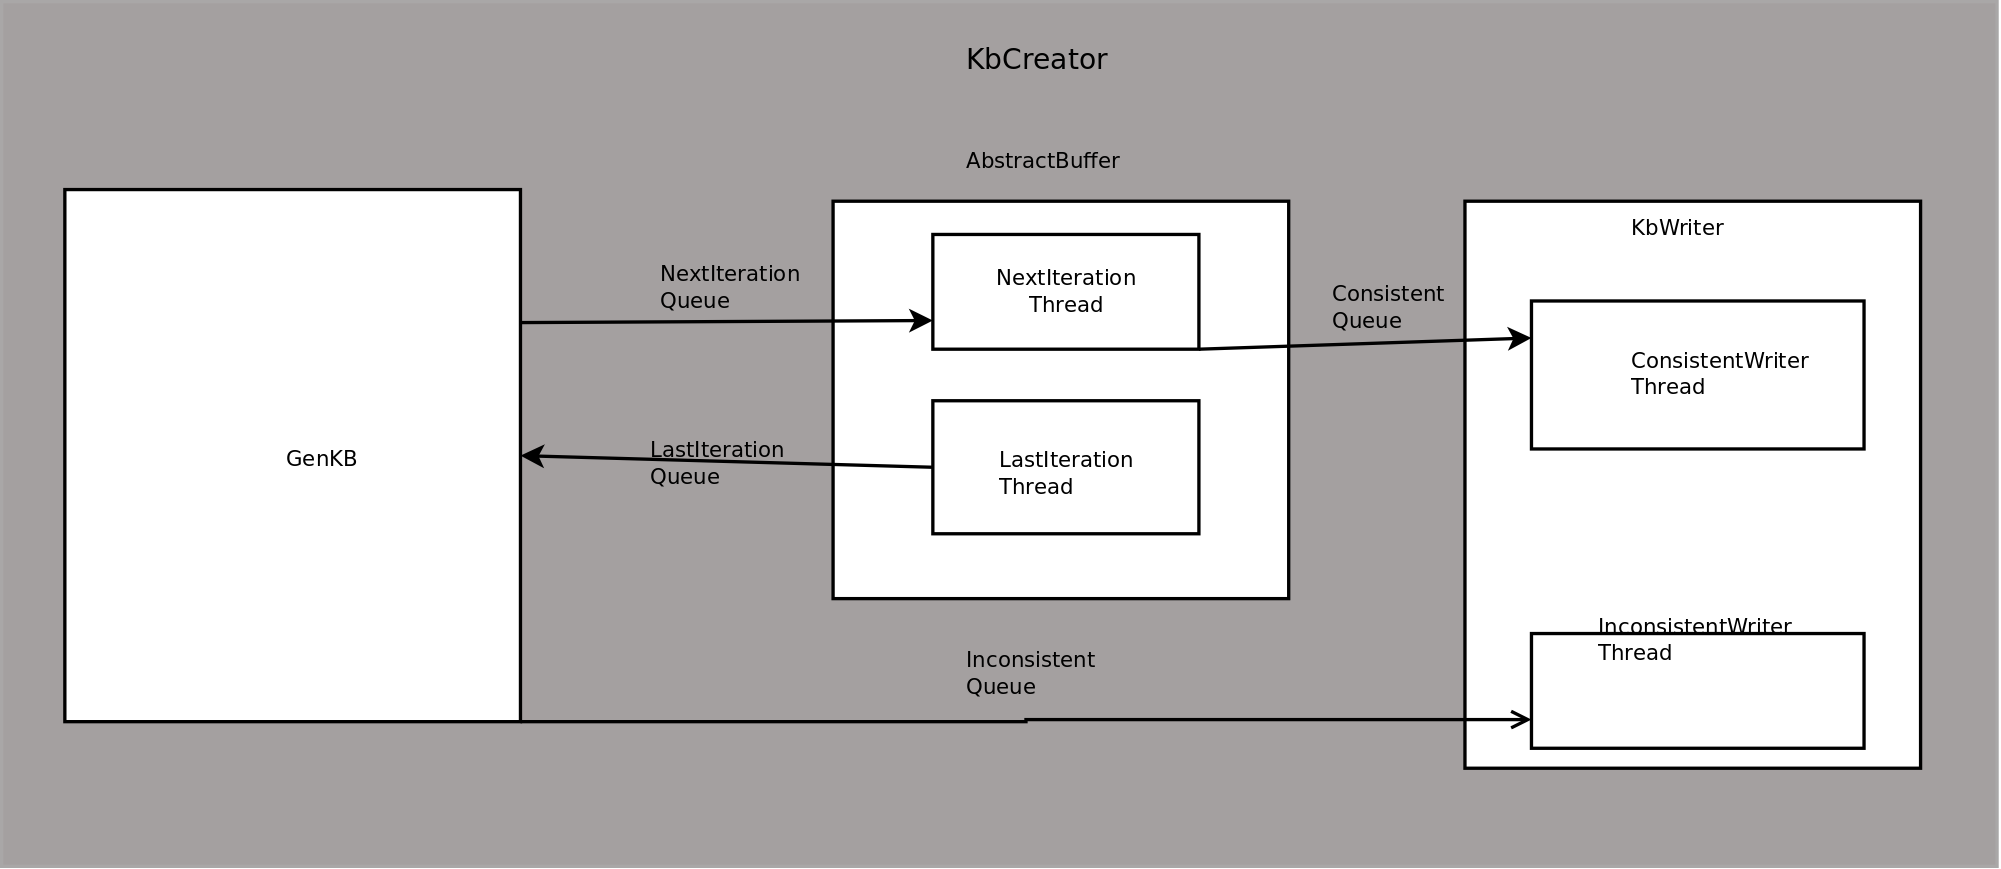
\includegraphics[width=1\linewidth]{bilder/kbcreator.png}
\caption{KbCreator Aufbau}
\label{pic:kbcreator}
\end{figure}



Die Generierung der Wissensbasen und damit der zentrale Teil dieser Arbeit ist schematisch in \autoref{pic:kbcreator} abgebildet. Alle beteiligten Elemente befinden sich im Package KbCreator. Es handelt sich dabei um drei Hauptbestandteile, die miteinander agieren. Diese tauschen dazu miteinander Daten aus, was hier mit Pfeilen dargestellt ist. Die Pfeilrichtung zeigt die Richtung, in der die Daten bewegt werden. Im Programm sind die Pfeile jeweils als Queues implementiert. Auf der linken  Seite befindet sich das GenKb Objekt. Dieses Objekt beinhaltet den Thread welcher den eigentlichen GenKB Algorithmus darstellt,von hier wird der ganze Ablauf kontrolliert. In der Mitte befindet sich der AbstractBuffer. Dieser bildet die Datenstruktur \glqq l \glqq \space aus GenKB ab: Eine Liste von Listen von Paaren aus Wissensbasen und Kandidaten, in Java Schreibweise List<List<Pair>>. In diesem AbstractBuffer befinden sich zwei Threads. Der LastIterationThread kümmert sich um die Bereitstellung der Paare aus Wissensbasen und Kandidaten der Iteration $k$ für GenKB. Der NextIterationThread nimmt die Paare der Iteration $k+1$ auf und kümmert sich um deren Speicherung. Auf der rechten Seite in der Abbildung befindet sich der KbWriter. Hier werden die erstellten fertigen Wissensbasen gespeichert. Das übernimmt jeweils ein Thread für die konsistenten und ein Thread für die inkonsistenten Wissensbasen. \\
Der Gedanke hinter dieser Architektur ist folgender: Der Thread GenKB ist der kritische Punkt bei der Generierung der Wissensbasen was die Geschwindigkeit angeht. Also soll so viel Arbeit wie möglich von GenKb in andere Threads ausgelagert werden um insgesamt eine möglichst hohe Geschwindigkeit zu erreichen.\\
In den folgenden Abschnitten werden die drei hier vorgestellten Teile als GenKkb, ZwischenSpeicherung der Daten und Speicherung der Wissensbasen genauer dargestellt.








\subsection{Implementierung von GenKb}
 

\begin{figure}
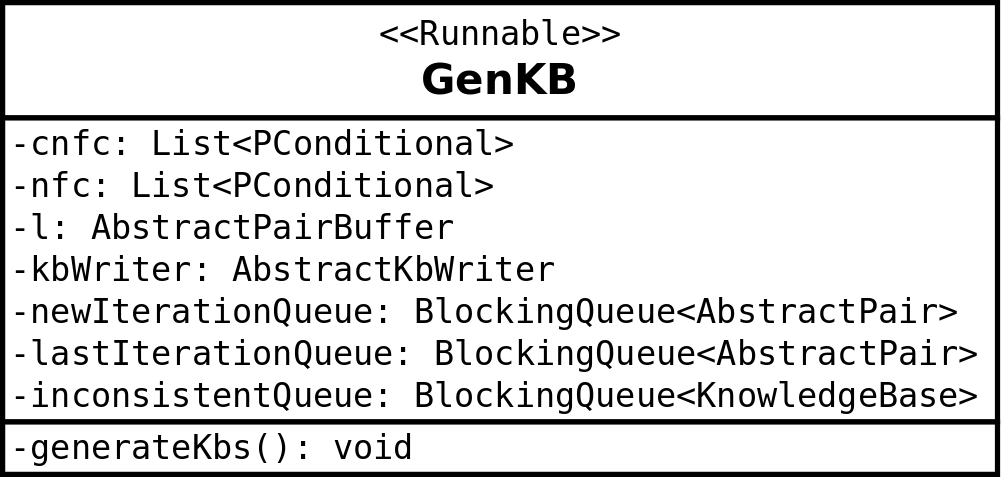
\includegraphics[width=0.5\linewidth]{bilder/genkb.png}
\caption{Klassendiagramm GenKb}
\label{pic:genkb}
\end{figure}



In diesem Abschnitt wird gezeigt, wie der konkrete Algorithmus GenKb aus \cite{beierle19} zur Generierung der Wissensbasen implementiert wurde. Wie schon erwähnt, befindet sich der Algorithmus in eigenem Objekt der Klasse GenKb, ein stark vereinfachtes Klassendiagramm dieses Objekts befindet sich in \autoref{pic:genkb}. Das Objekt implementiert das Java Interface \textit{Runnable} und kann somit als eigener Thread verwendet werden. Als Referenzen im Objekt befinden sich die Listen von PConditonals \textit{cnfc} und \textit{nfc}, die vom NfcCreator erstellt wurden und bereits erklärt wurden. Dann befindet sich eine Referenz auf das Objekt \glqq l\grqq \space, was dem \glqq l\grqq \space aus der Originaldarstellung von GenKb entspricht. Hauptsächlich ist es ein Objekt, was eine \textit{List<List<AbstractPair>>} beinhaltet, also die Paare aus \textit{<Konditional, Kandidaten>} während der Iterationen die Daten aufnimmt. Das Objekt \textit{kbWriter} kümmert sich um das persistente Schreiben der erstellten Wissensbasen auf einen Datenträger. Die Klassen AbstractPairBuffer und AbstractPairWriter werden in den nächsten Abschnitten beschrieben. Dann befinden sich im OBjekt noch drei Referenzen auf BlockingQueues: Die \textit{BlockingQueue<AbstractPair> newIterationQueue} nimmt die neu erstellten Paare aus <Wissensbasis, Kandidaten> auf und übergibt sie somit dem AbstractPairBuffer \textit{l}.
Von der \textit{BlockingQueue<AbstractPair> lastIterationQueue} werden die Paare entnommen, um sie in der aktuellen Iteration zu bearbeiten. Und die \textit{BlockingQueue<AbstractPair> inconsistentQueue} nimmt alle inkonsistenten Wissensbasen auf um die dem \textit{kbWriter} zu übergeben. \\
Im auf den folgenden zwei Seiten ist die konkrete Implementierung von GenKb gezeigt. Dabei werden mit Kommentaren in der Form \glqq //line 1\glqq \space die Entsprechung der folgenden Zeilen im Original gekennzeichnet. Nach dem dargestelltem Code folgt dessen Erläuterung.


\newpage
\begin{lstlisting}
private void generateKbs() throws InterruptedException {
    //line 1
    startIteration(0);

    //line 2
    k = 1;
    long consistentKbCounter = 1;
    long inconsistentKbCounter = 1;

    //line 3
    for (PConditional r : cnfc) {

        //line 4 and 5
        KnowledgeBase rKB = new KnowledgeBase(consistentKbCounter, r);
        consistentKbCounter++;
        List<PConditional> candidatesList = new ArrayList<>();
        for (PConditional conditional : nfc) {
            if (!(conditional.getEqConditionalsList().get(0).getNumber() < r.getNumber()))
                if (!(conditional.equals(r)))
                    if (!(conditional.equals(r.getCounterConditional())))
                        candidatesList.add(conditional);
        }
        newIterationQueue.put(new RealPair(rKB, candidatesList));
    }
    finishIteration(0);

    //line 6
    while (l.hasElementsForIteration(k)) {

        //line  7
        startIteration(k);
        consistentKbCounter = 1;
        inconsistentKbCounter = 1;

        //line 8
        while (l.hasMoreElementsForK(k)) {
            AbstractPair currentPair = lastIterationQueue.take();
            iterationPairCounter++;

            //line 9
            for (PConditional r : currentPair.getCandidatesList()) {

                //line 10
                if (currentPair.getKnowledgeBase().isConsistentWith(r)) {

                    //line 11 and 12
                    KnowledgeBase knowledgeBaseToAdd = new KnowledgeBase(consistentKbCounter, currentPair.getKnowledgeBase(), r);
                    consistentKbCounter++;
                    List<PConditional> candidatesToAdd = new ArrayList<>();
                    for (PConditional candidate : currentPair.getCandidatesList())
                        if (candidate.getNumber() > r.getNumber() && !candidate.equals(r.getCounterConditional()))
                            candidatesToAdd.add(candidate);

                    //line 12
                    newIterationQueue.put(new RealPair(knowledgeBaseToAdd, candidatesToAdd));

                } else {
                    inconsistentQueue.put(new KnowledgeBase(inconsistentKbCounter, currentPair.getKnowledgeBase(), r));
                    inconsistentKbCounter++;
                }
            }
            currentPair.clear();
        }

        //line 13
        finishIteration(k);
        k = k + 1;
    }
    finishAndStopLoop();
}
\end{lstlisting}


Die Methode \textit{void generateKbs()} ist im Gegensatz zum originalen GenKb keinen Rückgabewert. Stattdessen werden die Outputs, welche die Methode erzeugt, über drei BlockingQueues weitergegeben. Weiterhin kann die Methode eine InterruptedException werfen, nämlich genau dann wenn der Thread einen Iterrupt feststellt. Das passiert ausschließlich durch den Benutzer, wenn er den Stop Button der GUI betätigt, dann wird die InterruptedException gefangen und der Thread beendet.
 Ansonsten wurde versucht, die Methode nah am Orginal zu gestalten. Damit und der Kommentierung mit den Zeilennummern des Originals sollte die Methode möglichst selbst erklärend sein.\\
Zu Beginn wird in Zeile drei die Methode \textit{startIteration(0} aufgerufen. Mit dieser Methode wird immer die neue Iteration $k$ vorbereitet, insbesondere werden die Datenstrukturen \textit{l} und \textit{kbWriter} auf die neue Iteration initialisiert. Außerdem wird mit den beiden Methodenaufrufen die Zeitmessung für jede Iteration gestartet und das Ergebnis am Ende der Iteration in Sekunden in der Konsole ausgegeben. Diese Zeitmessung für Iterationen ist sehr nützlich als Benchmark um die Performance zu messen. Hier wird die Iteration 0 gestartet, das entspricht der Iteration zur Initialisierung der Wissensbasen. Auch alle anderen Iterationen werden durch die Methode \textit{startIteration(int k)} gestartet, so entspricht diese Methode dann der Code Zeile 7 des Originals. In den Zeilen 6 und 7 werden die beiden Zähler für die konsistenten und inkonsistenten Wissensbasen initialisiert. Sie sind im späteren Verlauf dafür da, das alle Wissensbasen Innerhalb einer Iteration eine eindeutige Nummer bekommen. Die Zähler sind bewusst als Datentyp \textit{long} gesetzt, da der Integer Datentyp sonst \textit{nur} maximal bis 2.147.483.647 zählen könnte, eine Grenze, die im Programm bei entsprechend langer Laufzeit durchaus erreicht werden könnte. \\
Die Initialisierung der Wissensbasen mit je einem Element funktioniert folgendermaßen: In Zeile 11 wird dazu über alle Konditionale aus \textit{cnfc} iteriert, was exakt der Zeile 3 des Originals entspricht. In Zeile 14 wird dann jeweils die Wissensbasis mit einem erstellt. In Zeile 16-21 wird nun dafür die Liste der Kandidaten erstellt. Dazu wird in Zeile 17 über alle Konditionale aus \textit{nfc} iteriert und im folgenden wird anhand von drei Ausschlusskriterien geprüft, ob das Konditional zu den Kandidaten gehören soll. In Zeile 18 werden alle Konditionale ausgeschlossen, die zu einer Äquivalenzklasse gehören, dessen kanonischer Vertreter kleiner als das Konditional $r$ ist. In Zeile 19 wird das Konditional $r$ selbst ausgeschlossen und in  Zeile 20 wird das Counter Conditional ausgeschlossen. Wenn alle diese 3 Ausschlusskriterien auf das \textit{nfc} element nicht zutreffen, wird es in Zeile 21 zur Liste der Kandidaten hinzugefügt. In Zeile 23 wird dann das neue Paar in die \textit{newIterationQueue} eingefügt. Die Initialisierung endet in Zeile 25 mit dem Methodenaufruf um die Iteration 0 u beenden. \\
In Zeile 28 läuft dann die Schleife für alle weiteren Iterationen, die Zeile entspricht so exakt Zeile 6 des Originals. In Zeile 31 wird die Iteration $k$ vorbereitet, was Zeile 7 des Originals entspricht. Anschließend werden die Zähler für die Wissensbasen in Zeile 32 und 33 initialisiert. \\
Die Schleife ab Zeile 36 läuft so lange wie für die aktuelle Iteration $k$ weitere Paare bereit stehen, das entspricht Zeile 8 des Originals. Dazu wird in Zeile 37 das nächste Paar abgerufen und in der Variable \textit{currentPair} gespeichert, die Zählervariable anschließend um den Wert 1 erhöht. \\
In Zeile 41 wird dann über alle Konditionale der Kandidatenliste des aktuellen Paars iteriert, das entspricht Zeile 9 des Originals. In Zeile 44 wird dann geprüft, ob die Wissensbasis des aktuellen Paars konsistent mit dem Kandidaten \textit{r} ist, analog Zeile 10 des Originals. Sind diese konsistent, wird in Zeile 47 eine neue Wissensbasis aus diesen beiden erstellt. In Zeile 49 - 52 wird dann die Liste der Kandidaten für das neue Paar gebildet. Dazu werden alle Kandidaten der Kandidaten von \textit{currentPair} eingeschlossen, falls sie kleiner sind als \textit{r} und nicht dem Counter Conditional von \textit{r} entsprechen. In Zeile 55 wird dann aus der neuen Wissensbasis und der neuen Kandidatenliste ein neues Paar gebildet und dieses der \textit{newIterationQueue} hinzugefügt. \\
In Zeile 62 wird die Methode \textit{clear()} auf \textit{currentpair} ausgeführt. Da diese Referenz  an diesem Zeitpunkt nicht mehr gebraucht wird, kann so viel Arbeitsspeicher wieder freigegeben werden. Wäre dieser Aufruf nicht hier, würde dieser Speicher erst wesentlich später freigegeben. In Zeile 66 und 67 wird dann die Iteration $k$ kontrolliert beendet und es wird gewartet, bis die anderen Threads die Iteration fertig gestellt haben. Anschließend wird $k$ um 1 erhöht, was Zeile 13 des Originals entspricht. Wenn der Algorithmus fertig ist, werden mit dem Methodenaufruf Zeile 69 die Threads kontrolliert beendet und der Ablauf ist fertig. \\
Der Grund, warum in die Listen der Kandidaten in Zeilen 4 und 11 des Originals hier nicht mit der Menge \textit{D} gebildet werden, ist die Performance. Die Zeile 11 ist kritisch, was die Performance angeht, da sie sich im der innersten Schleife befindet. Mit der Implementierung wie hier soll einfach vermieden werden, dass für jeden Kandidaten eine neue Liste erstellt wird, die direkt danach wieder gelöscht wird. Die eigentliche Funktion bleibt die selbe, alle Elemente, die in \textit{D} enthalten wären, werden als Kandidaten ausgeschlossen. In Zeile 4 wäre die Performance unwichtig, aber sie ist der Einheitlichkeit halber ähnlich wie Zeile 11 gestaltet.

\subsection{Zwischenspeicherung der Daten}
In diesem Abschnitt wird beschrieben, wie die Arbeitsdaten von GenKB verwaltet und gespeichert werden. Während einer Iteration $k$ werden Daten von Iteration $k$ verarbeitet und neue Daten unter $k + 1$ abgelegt. Dadurch entstehen große Mengen von Daten, welche bis zur jeweils nächsten Iteration behalten werden müssen. Dabei stellt sich schnell heraus, dass es für den Erfolg des ganzen Programms kritisch ist, diese Daten so effizient und sparsam wie möglich zu verwalten. \\
In der Originalversion von GenKB wird diese Datenstruktur als \glqq L\grqq \space bezeichnet, bearbeitet werden in einer Iteration $k$ jeweils $L_k$ und  $L_{k+1}$. Die Datenstruktur ist im Prinzip eine Liste die für jedes Element $L_k$ wieder eine Liste mit dem Datensätzen für die jeweilige Iteration beinhaltet. Diese Struktur wird hier folgendermaßen dargestellt: Einzelne Datensätze werden dabei als Objekte gespeichert, welche jeweils eine Wissensbasis und eine Menge an Kandidaten enthalten. Die Verwaltung dieser Datensätze übernimmt ein Puffer, der die Daten Wahlweise entweder im Arbeitsspeicher oder auf der Festplatte speichert und rechtzeitig zur Verfügung stellt. Um die große Menge der Daten besser handhaben zu können, werden die Datensätze dabei jeweils zur Speicherung komprimiert und vor der Benutzung wieder rekonstruiert.

\subsubsection{Paare aus Wissensbasis und Kandidaten}
Als \textit{Paare} wird im Folgenden die Einheit aus einer ursprünglichen Wissensbasis und der zugehörigen Menge an Konditionalen als Kandidaten bezeichnet, um welche die ursprüngliche Wissensbasis möglicherweise erweitert werden kann. Im Algorithmus GenKB in \cite{beierle19} werden diese Paare in Zeile 5 initialisiert und in Zeile 8ff bearbeitet. Dargestellt wird diese Einheit mit charakteristischen dreieckigen Klammern in der Form $<R, C>$, was im Folgenden bei Gelegenheit auch so beibehalten wird. \\
Im Programm werden zwei Implementierungen zur Repräsentation dieser Paare genutzt, welche hier vorgestellt werden. Beide erben von  der Klasse \textit{AbstractPair}, was die einige Gemeinsamkeiten beider Varianten vereint und ansonsten die Schnittstelle der Paare bildet. Die beiden Implementierungen unterscheiden sich hauptsächlich in der Art der Speicherung der Kandidaten. Da davon sehr viele verwaltet werden müssen, machen sie den allergrößten Teil des Speicherverbrauchs eines Paares aus. Die erste Implementierung ist \textit{RealPair}, hier werden die Kandidaten als Liste von Konditionalen verwaltet. Das ist naheliegend, einfach und schnell, benötigt aber sehr viel Arbeitsspeicher. Die zweite Implementierung \textit{CompressedPair} komprimiert die Liste der Kandidaten und spart dadurch viel Arbeitsspeicher, ist dafür jedoch langsamer. Im späteren Programmablauf arbeitet GenKB selbst mit RealPairs. Die Klasse CompressedPair bietet dann die Möglichkeit den Speicherbedarf zu reduzieren, wenn die Daten im Arbeitsspeicher zwischengespeichert werden sollen. Wenn die Daten auf der Festplatte gespeichert werden, wird dazu ein ähnlnlicher Kompressionsmechanismus wie in CompressedPair angewandt.




\paragraph{Abstract Pair}
\label{sec:abstractpair}

\begin{figure}
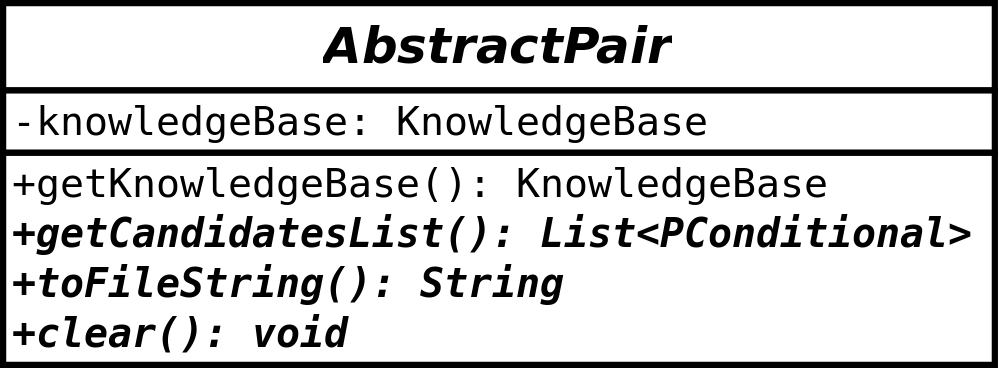
\includegraphics[width=0.45\linewidth]{bilder/AbstractPair.png}
\caption{AbstractPair}
\label{pic:abstractpair}
\end{figure}


Wie bereits beschrieben, vereint die Klasse AbstractPair die Gemeinsamkeiten ihrer beiden Implementierungen und bildet die Schnittstelle für deren Verwendung. Ein etwas vereinfachtes Diagramm der Klasse AbstractPair ist in \autoref{pic:abstractpair}  zu sehen. Als Instanzvariable besitzt die Klasse nur eine Wissensbasis in Form eines \textit{KnowledgeBase} Objekts und als Klassenattribut eine Map<Integer,PConditional> mit der alle Konditionale von NFC unter ihrer Nummer aufrufbar sind. Des Weiteren besitzt die Klasse zwei abstrakte und zwei konkrete Methoden. Die Methoden \textit{getKnowledgeBase()} und \textit{ getCandidatesList()} sind selbsterklärend. Die \textit{toFileString()} Methode gibt einen String zurück der die Klasse in einen String transformiert um diesen auf der Festplatte zu speichern, welcher im nächsten Absatz genauer erklärt wird. Die letzte Methode \textit{clear()} ist dazu da Speicher zu sparen und löscht die Daten in der Klasse, wenn diese nicht mehr gebraucht werden. Die \textit{clear()} Methoden in den Pair Implementierungen funktionieren nach folgendem Prinzip: Der Speicherbedarf eines Pairs wird zum Großteil von den enthaltenen Instanzvariablen bestimmt. Diese Variablen werden einfach nach dem Schema \textit{variable = null} "gelöscht". Genau genommen wird dadurch Referenz von Objekt auf \textit{null} geändert. Dadurch kann der \textit{Java Garbage Collector} erkennen, dass das Objekt selbst nicht mehr referenziert wird und wird es bei Gelegenheit löschen. Zumindest, falls es auch sonst nirgendwo mehr referenziert wird.

\begin{figure}
\begin{lstlisting}
KB
1{1}
C
3-6050
END
\end{lstlisting}
\caption{\textit{RealPair} als String zum Speichern auf der Festplatte}
\label{code:pair-text}
\end{figure} 

Die größte Komplexität der Klasse AbstractPair liegt darin, alle Informationen eines Pairs in einen möglichst kurzgefasstes Stück Text umzuwandeln und später aus diesem Stück Text auch wieder das Objekt zu rekonstruieren. Diese Funktion wird gebraucht, um die Daten auf der Festplatte abzulegen. Die Repräsentation des Pairs als Text muss zum Einen kurz sein, um die Speicherung und das Lesen zum beschleunigen. Zum Anderen werden so viele dieser Objekte gespeichert, dass auch der Gesamtverbrauch an Speicher relevant ist. In \autoref{code:pair-text} ist die Repräsentation des allerersten Pairs abgebildet, welches GenKB mit der Signatur $\Sigma_{abc}$  erstellt. In Zeile 1 ist mit KB einfach die Information kodiert, dass als nächstes die KnowledgeBase beschrieben wird. Die Beschreibung der Wissensbasis in Zeile 2 zeigt als erstes die Nummer vor der Klammer, welche die Nummer der Wissensbasis repäsentiert und hier 1 lautet. Dahinter, innerhalb der geschweiften Klammern, befindet sich die Menge der Konditionale innerhalb der Wissensbasis, hier ebenfalls die Nummer 1. Mehrere Konditionale würden durch Kommas getrennt aufgeführt. Das C in Zeile 3 kündigt an, dass als nächstes die Liste der Kandidaten folgt. In Zeile 4 dann die komprimierte Liste der Kandidaten, die etwas erklärungsbedürftig ist. Sie wird hier so interpretiert, dass alle Konditionale mit den Nummern 3-6050 in die Liste der Kandidaten aufgenommen werden sollen. Dazu werden bei der Rekonstruktion die Konditionale aus der Map<Integer, PConditional> aus AbstractPair abgerufen und in die Liste der Konditionale eingefügt. Das ist in diesem Beispiel sehr einfach, da sich in der Menge keine Lücken befinden. Wenn sich Lücken darin befinden, werden die einzelnen zusammenhängenden Bereiche von Kommas getrennt. Beispielsweise bedeutet "3-5, 7-6050" \space dass alle Konditionale außer den Nummern 1,2 und 6 in die Liste der Kandidaten aufgenommen werden sollen. Hier wird offensichtlich, dass die Effizienz dieser Speicherung dann besonders hoch ist, wenn kaum Lücken vorhanden sind. Das ist in GenKB bei niedrigen Werten für k der Fall. Mit steigendem k steigt auch die Menge der Lücken und damit der Speicherbedarf für die Repräsentation des Pairs. Da jedoch aufgrund der Geschwindigkeit sowieso nur geringe Werte von k relevant sind, ist damit eine sehr effiziente Speicherung ausreichend sichergestellt. In Zeile 5 des Beispiels hat der Eintrag END die Bedeutung, dass das Paar hier endet. Dadurch werden die verschiedenen Paare innerhalb einer Datei voneinander getrennt. Da während des Programmablaufs sehr viele Paare erstellt werden, wäre es ineffizient, für jedes Paar eine eigene Datei zu erstellen. Das Schreiben der einzelnen Dateien auf die Festplatte wäre dann der Flaschenhals für die Geschwindigkeit. Deshalb werden sehr viele Paare in eine einzelne Datei zusammengefasst. Wie viele genau das sind, kann über die GUI des Programms bestimmt werden. Mehr dazu später auch \autoref{sec:pairbuffer}. Analog zur Speicherung eines Pairs als String besitzt dann die Implementierung RealPair auch einen Konstruktor \textit{RealPair(String string)}, der ein Objekt der Klasse aus einem solchen String wieder erzeugen kann.

\paragraph{Real Pair}
\label{sec:realpair}
Die Klasse \textit{RealPair} speichert die Liste der Kandidaten zur Erweiterung der enthaltenen Wissensbasis als ArrayList<PConditional>. Das ist in der Verarbeitung schnell, benötigt jedoch sehr viel Speicher. Während des Programmablaufs existiert deshalb zu jedem Zeitpunkt nur eine kleine Menge an Objekten dieser Klasse. Dadurch ist der hohe Speicherbedarf unproblematisch und die gute Verarbeitungsgeschwindigkeit kann genutzt werden. \\
Es existieren drei Konstruktoren der Klasse RealPair. Ein einfacher Konstruktor in Form von \textit{RealPair(KnowledgeBase knowledgeBase, List<PConditional> candidates)} wird dazu verwendet, um das Paar in GenKB in Zeile 5 und 12 zu erstellen. In dieser Form wird das RealPair Objekt dann zur Weiterverarbeitung im PairBuffer wie unter \ref{sec:pairbuffer} beschrieben übergeben. Ein weiterer Konstruktor dieser Klasse steht in der Form \textit{RealPair(AbstractPair other)} bereit. Dieser erstellt aus einer AbstractPair Implememtierung ein RealPair. Dieser Konstruktor wird dazu genutzt, um aus einem CompressedPair ein RealPair zu erzeugen, also die komprimierten Daten wieder zu entpacken. Ein dritter Konstruktor besteht in der Form \textit{RealPair(String string)} zur Verfügung. Mit diesem kann wie in \autoref{sec:hddBuffer} beschrieben ein RealPair aus einem Stück Text rekonstruiert werden.


\paragraph{Compressed Pair}
Die Klasse  \textit{CompressedPair} ist die Implementierung von AbstractPair, die verwendet wird, wenn die Daten möglichst platzsparend im Arbeitsspeicher gehalten und werden sollen. Wie der Name schon verrät, ist dafür ein Kompressionsmechanismus eingebaut. Dieser betrifft die Speicherung der Liste der Kandidaten. Ähnlich wie bei der Speicherung in AbstractPairs als Text auf der Festplatte durch die Methode \textit{toShortFileString()} werden hier zusammenhängende Folgen von Konditionalen genutzt, um Speicherplatz zu sparen. Dazu besitzt die Klasse CompressedPair ein zweidimensionales Array in der Form $int[][]$. Damit werden die Daten im Arbeitsspeicher abgelegt. Die Wahl des Datentyps fällt auf Arrays statt Listen, da die Speicherung hier viel effizienter erfolgen kann. In Java existiert der simple Datentyp int und analog dazu die Möglichkeit Integer Werte als Objekte der \textit{Integer} Klasse zu speichern. Der simple int Typ benötigt dabei jedoch deutlich weniger Speicher als der Overhead eines Objekts der Klasse Integer. Listen können in Java jedoch nur von Integer Objekten erstellt werden, nicht von simplen int Werten, daher müssen die Werte hier in Arrays gespeichert werden.\\
Der Kompressionsalgorithmus sucht wieder zusammenhängende Mengen von Konditionalen im Format [Nummer des ersten Konditionals] [Nummer des letzten Konditionals]. Diese werden als int Array mit der Länge zwei abgelegt. Von diesen int Arrays der Länge zwei wird dann wiederum Array erstellt und darin die gesamte Menge der Konditionale gespeichert. Die Größe des gesamten Arrays beträgt dann [Menge der zusammenhängenden Bereiche][2]. Solange die zusammenhängenden Bereiche groß sind, funktioniert die Kompression sehr gut. Mit steigendem Wert von k kommen jedoch immer mehr Lücken hinzu und die Speicherung wird zunehmend umständlich. \\
Mit der Signatur $\Sigma_{abc}$ werden nur geringe Werte für k erreicht, demzufolge ist die Speicherung im relevanten Bereich sehr effizient. Mit der Signatur $\Sigma_{ab}$ werden jedoch höhere Werte für k erreicht. Zusätzlich ist hier die Menge der Kandidaten viel geringer, sodass diese Kompression kaum Vorteile bringt. Das ergibt dann den folgenden Effekt: Für geringe Werte für k wird weniger Speicher benötigt, für hohe Werte für k wird sogar mehr Speicher benötigt im Vergleich zum Verzicht auf Kompression. Da die Signatur $\Sigma_{abc}$ im Vordergrund steht wird die Ineffizienz für $\Sigma_{ab}$ für hohe Werte für $k$  jedoch ignoriert.\\
Als Konstruktor für die Klasse wird nur der Konstruktor in der Form \textit{CompressedPair( AbstractPair originalPair)} verwendet. Damit werden im \textit{CompressedRamBuffer} wie in \autoref{sec:compressedrambuffer} beschrieben RealPair Objekte in CompressedPair Objekte umgewandelt, um Speicherplatz zu sparen.


\subsubsection{Speicherung der Paare}
\label{sec:pairbuffer}

Die Datenstruktur, welche die im Abschnitt zuvor beschriebenen Paare aus Wissensbasis und Kandidaten verwaltet, ist Thema dieses Abschnittes und wird im Folgenden auch als  \textit{PairBuffer} bezeichnet. Der PairBuffer ist damit das Element, welches in GenKb mit der Variable groß $L$ bezeichnet wird. dafür sind im Programm drei verschiede Varianten implementiert: Zwei Optionen legen die Daten im Arbeitsspeicher ab, davon eine Variante mit Kompression der Daten und eine ohne solche Kompression. Die dritte Variante verwendet als Speicher die Festplatte. Alle drei Varianten besitzen zwei eigene Threads, die der eigentlichen GenKB Implementierung so viel wie möglich Arbeit abnehmen. Der Nutzer kann in der grafischen Oberfläche in den Optionen unter \glqq Buffering\grqq \space wählen, welche der Varianten verwendet werden soll. \\
Von den drei angesprochenen Varianten  sind \textit{CompressedRamBuffer} und \textit{HddBuffer} die Beiden, die sich als gut funktionierend dargestellt haben. Der SimpleRamBuffer ist wegen seines enormen Speicherverbrauchs nur wenig praktikabel und hauptsächlich noch zu Demonstrationszwecken implementiert.

\paragraph{AbstractPairBuffer}
\label{sec:abstractbuffer}

\begin{figure}
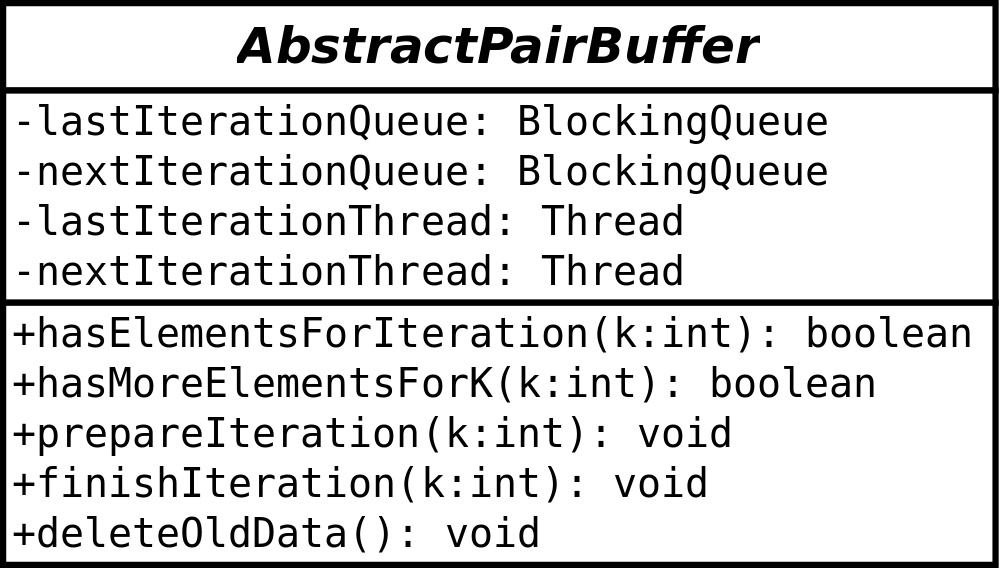
\includegraphics[width=0.45\linewidth]{bilder/AbstractPairBuffer.png}
\caption{AbstractPairBuffer}
\label{pic:abstractpairbuffer}
\end{figure}


\textit{AbstractPairBuffer} ist die Klasse, von welche alle Varianten der Speicherverwaltung erben und hat dabei hauptsächlich den Charakter eine Schnittstelle. Ein vereinfachtes Klassendiagramm ist in \autoref{pic:abstractpairbuffer} zu sehen. Die Klasse besitzt zwei BlockingQueues als Instanzvariablen zur Verwaltung der Pairs, welche allerdings erst in den Implementierungen konkret initialisiert werden.  BlockingQueues deshalb, weil sie erstens threadsicher sind und zweitens das im Anschluss beschriebene Blocking unterstützen. Die erste Queue heißt \textit{lastIterationQueue} und stellt  die Paare zur Verarbeitung in einer Iteration $k$ bereit. Die zweite heißt \textit{nextIterationQueue} und nimmt während einer Iteration $k$ die für die nächste Iteration $k+1$ erstellen Paare. Um diese Weiterverarbeitung der Paare in den Queues kümmert sich dann jeweils ein eigener Thread innerhalb des AbstractPairBuffers, namentlich \textit{lastIterationThread} und \textit{nextIterationThread}. \\
Beide Queues werden als Objekte der Klasse \textit{ArrayBlockingQueue} mit fester Größe initialisiert, diese Implementierung hat sich für die Aufgabe nach einigen Tests als gute Wahl erwiesen. Die andere Möglichkeit wäre gewesen, stattdessen eine \textit{LinkedBlockingQueue} einzusetzen. Beide bieten die selben hier benötigten Features. Intern setzt die eine Variante auf ein Array, die andere auf eine LinkedList. Zum Vergleich wurden beide Varianten implementiert und als Benchmark die Zeit für die erste Iteration mit Signatur $\Sigma_{abc}$ gemessen. Das Ergebnis zeigte, dass die Zeit für beide Varianten überraschenderweise bis fast identisch war: Die ArrayBlockingQueue benötigte bei den Tests im Durchschnitt 277 Sekunden, die LinkedBlockingQueue 277 Sekunden. Allerdings war der Speicherverbrauch der ArrayBlockingQueue wesentlich geringer, daher wurde dieser Implementation vorgezogen. \\
Dadurch, dass die \textit{lastIterationQueue} und die \textit{nextIterationQueue} mit fester Größe initialisiert werden wird sichergestellt, dass die Queues nicht endlos groß Wachsen können. In Java sind BlockingQueues mit fester Größe gut geeignet, um Consumer-Producer Szenarios  mittels Threads umzusetzen. Wenn eine solche Queue voll ist, wartet ein Producer Thread automatisch, bis wieder ein Platz frei wird, um dann das nächste Element abzulegen. Analog wartet ein Thread automatisch, wenn er ein Element aus der Queue entnehmen will, diese jedoch im Moment keine Elemente beinhaltet. Dieser Thread läuft erst dann weiter, wenn wieder ein Element bereitgestellt wurde. Dadurch sorgen die Queues dafür, dass Producer und Consumer aufeinander warten und dabei ineffizientes \textit{busy wait} vermeiden.\\
Im Falle der \textit{lastIterationQueue} ist der Thread von GenKB in der Rolle des Consumers, welcher die Pairs konsumiert und weiterverarbeitet. Der Thread im PairBuffer legt die Pairs in der Queue bereit und ist damit der Producer. Bei der \textit{nextIterationQueue} verhält es sich genau anders herum: GenKB erstellt die Pairs als Producer und legt sie in der Queue ab, während der Thread im PairBuffer der Consumer ist und die Pairs der Queue entnimmt. Die beiden Queues werden von der Implementierung von GenKB wie folgt verwendet: Die \textit{lastIterationQueue} stellt die Pairs aus Iteration $k$ bereit, damit GenKB sie nacheinander entnehmen und bearbeiten kann. Das entspricht der Zeile 8 im Algorithmus. Die \textit{nextIterationqueue} nimmt die neu erstellten Paare in GenKB auf, das entspricht den Schritten in Zeile 5 und 12. Die Implementierung von GenKB greift dann also nicht auf den PairBuffer selbst zu, sondern beide Teilen sich die Queue und tauschen die Daten darüber aus. \\
Die Methoden der Klasse AbstractPairBuffer sind allesamt abstrakt. Das sind zum einen zwei Methoden für die Loops in GenKB. Das ist \textit{hasElementsForIteratin(k)}, was der GenKb Zeile 6 entspricht. Dann noch die Methode \textit{hasMoreElementsForIteration(k)}, diese entspricht dem Loop in Zeile 8 in GenKB. Dann noch die zwei Methoden \textit{prepareIteration(int k)} und \textit{finishIteration(int k)}, die einfach die Iterationen für das übergebene $k$ vorbereiten oder abschließen. Eine wichtige Methode ist noch \textit{deleteOldData(int k)}. Sie wird aufgerufen, um die Daten einer alten Iteration zu löschen, die nicht mehr gebraucht werden. Dadurch wird der dafür belegte Speicherplatz wieder freigegeben. Dazu kommen noch ein paar Methoden, die nicht im Diagramm gezeigt sind. Das sind insbesondere Getter für die grafische Oberfläche und eine Methode zum außerplanmäßigem Beenden der Threads, wenn in der GUI der Stop Button betätigt wurde.



\paragraph{CompressedRamBuffer}\mbox{}
\label{sec:compressedrambuffer}

Der RamPairBuffer besitzt eine Datenstruktur in der Form \textit{List<List<CompressedPair>>} und zwei dazugehörige Threads dafür. Die Threads stellen die Verbindung zwischen der Datenstruktur und den beiden BlockingQueues dar, die von GenKB verwendet werden. \\
Ein Thread kümmert sich um die \textit{nextIterationQueue}, also um die von GenKB in Zeile 5 und 12  neu erstellten Paare in Form von Instanzen der Klasse RealPair. Sobald die \textit{nextWiterationQueue} Pairs enthält, entnimmt der Thread die Pairs und wandelt diese in CompressedPairs um. Dazu Wird der Konstruktor \textit{CompressedPair(RealPair)} genutzt. Die neu erstellen CompressedPairs werden dann in die Datenstruktur in der Liste unter dem aktuellen Wert für $k+1$ abgelegt. Diese Kompression findet in dem  dedizierten Thread statt und nicht in der Impelementierung von GenKb selbst, weil das GenKB eine Menge Arbeit abnimmt und somit merklich beschleunigt. \\
Analog dazu kümmert sich der andere Thread um die \textit{lastIterationQueue}. Der Thread befüllt die Queue mit RealPairs, damit sie GenKB in Zeile 9 entnehmen kann und nicht selbst entkomprimieren muss. Auch das beschleunigt GenKB selbst deutlich. Der Thread entnimmt also die CompressedPairs aus der Liste mit Index $k$, wandelt sie duch den Konstruktor \textit{RealPair(CompressedPair)} um und legt sie in die \textit{lastIterationQueue}. \\
Die beiden Queues werden jeweils als \textit{ArrayBlockingQueue(1000)} mit der Größe 1000 initialisiert. Die genaue Größe ist nicht wirklich wichtig. Sie ist mit dem Wert 1000 groß genug, dass sie den Prozess nicht verlangsamt, aber auch nicht so groß dass sie zu viel Speicher benötigen würde. \\
Die Liste in der Form \textit{List<List<CompressedPair>>} wird von einigen Methoden zum Iterationswechsel bearbeitet. Dazu wird beispielsweise durch die \textit{prepareIteraiton(int k)} Methode eine neue Liste für k angelegt. Die \textit{finishIteration(int k)} Methode sorgt dafür, dass alle Pairs aus den Queues auch fertig bearbeitet werden, bevor die neue Iteration beginnt. Dadurch wird ausgeschlossen, dass durch den Iterationswechsel Datensätze verloren gehen können. \\
Die \textit{deleteOldData(int k)} Methode löscht dann in der List<List<CompressedPair>> das Element $k-1$ um den Speicherplatz wieder freizugeben.


\paragraph{SimpleRamBuffer}\mbox{}
\label{sec:simplerambuffer}

Bei dieser Option werden die Daten einfach in einer Datenstruktur in der Form \textit{List<List <RealPair>>} im Arbeitsspeicher gehalten. Das ist die naheliegendste Variante und gleichzeitig diejenige, die am wenigsten praktikabel ist. Der Speicherverbrauch ist enorm und schon nach kurzer Zeit bricht das Programm mit einem \textit{Out of Memory Error} ab. \\
Der SimpleRamBuffer ist daher eigentlich kaum geeignet für den produktiven Einsatz. Er bietet keine Vorteile gegenüber dem CompressedRamBuffer, dafür den großen Nachteil des erheblichen Speicherverbrauchs. Intern erbt deshalb die Klasse SimpleRamBuffer von CompressedRamBuffer und überschreibt nur wenige Dinge, um statt CompressedPairs RealPairs zu verwenden. Der Rest ist identisch mit dem CompressedRamBuffer aufgebaut, deshalb entfällt an dieser Stelle die Erklärung der internen Funktionsweise, es wäre nur eine Wiederholung vom vorhergehenden Absatz. \\



\paragraph{HDDPairBuffer} \mbox{}
\label{sec:hddBuffer}


Die Klasse \textit{HddPairBuffer} ist die Implementierung des AbstractPairBuffers, welche die Paare auf der Festplatte zwischenspeichert. Damit kann die Begrenzung der anderen Varianten durch den typischerweise recht knappen Arbeitsspeicher umgangen werden. Dabei müssen die Paare immer in der richtigen Reihenfolge bleiben und es darf kein Paar verloren gehen oder mehrfach verarbeitet werden. Auch die Iterationen selbst müssen alle vollständig und ohne Überlappungen sauber getrennt voneinander ablaufen. Zusätzlich werden durch den HddPairBuffer der GUI noch ein paar Statusinformationen bereitgestellt.\\
Die GUI bietet im Optionenfeld an, einige Einstellungen für den HddPairBuffer zu treffen: \textit{Delete temporary files} ist standardmäßig gesetzt und sorgt dafür, dass die nicht mehr benötigten Daten von der Festplatte automatisch gelöscht werden. Wird die Option deaktiviert, werden die Dateien nicht mehr automatisch gelöscht und können vom Benutzer betrachtet werden. Des Weiteren kann die Menge der Pairs eingestellt werden, welche maximal  zusammen in eine Datei geschrieben werden. Voreingestellt sind hier 80.000. \\
Die Dateien werden beim Schreiben während einer Iteration nach dem Namensschema $0, 1, 2, ...$  als Dateinamen benannt. Genau nach diesem Schema werden die Dateien auch wieder eingelesen. Dazu prüft der lesende Thread zunächst, wie viele Dateien sich im zu lesenden Ordner befinden. Er hat dann eine Integer Zähler Variable, welche mit 0 initialisiert und nach jedem Lesen um 1 erhöht wird. Das läuft, bis die Zählervariable die maximale Anzahl der Dateien erreicht hat. Dadurch ist sichergestellt, dass alle Dateien gelesen werden und das sie dabei auch genau in der Reihenfolge gelesen werden, in der sie abgelegt wurden. \\
Im Zuge der Einstellung der maximalen Anzahl von Pairs pro Datei wird indirekt die Größe der beiden BlockingQueues \textit{lastIterationqueue} und \textit{nextIterationQueue} eingestellt. Beide werden auf den Doppelten Wert der maximalen Pairs pro Datei initialisiert, denn diese Queues arbeiten eng mit dem Lesen und Schreiben der Dateien zusammen. Insbesondere muss vermieden werden, dass die \textit{nextIterationqueue} kleiner ist als die Menge der Pairs pro File, da hier sonst ein Lock entstünde, den das Programm nicht mehr auflösen könnte. Wenn die Queues einfach deutlich größer sind als die Menge der Pairs pro Datei werden hier im Voraus alle potentiellen Probleme vermieden. \\
Der HDDPairBuffer beinhaltet zwei Threads: Der \textit{nextIterationThread} nimmt die neu erstellen Paare der Iteration $k+1$ auf und schreibt sie auf die Festplatte. Dazu beobachtet der Thread die Größe der Queue. Wenn diese entweder die maximale Anzahl der Pairs for Datei erreicht hat, oder eine Iteration beendet werden soll, legt er eine neue Datei an und schreibt in diese die Pairs hinein. Der \textit{lastIterationThread} liest die Paare der Iteration $k-1$ von der Festplatte und stellt sie GenKB bereit in dem er sie die \textit{lastIterationQueue} als RealPair Instanzen einfügt. Dadurch, dass der Festplattenzugriff auf diese zwei Threads in Lesen und Schreiben aufgeteilt wird, wird vermieden, dass sich diese beiden Aufgaben gegenseitig behindern können. \\
Zum Iterationswechsel überschreibt die Klasse HddPairBuffer die Methode \textit{prepareIteraion(int k)}. Damit wird der Unterordner auf der Festplatte angelegt, in dem die Daten der Iteration gespeichert werden. Ebenfalls werden die beiden Threads initialisiert. Auch die Methode \textit{finishIteration(int k)} wird von HddPairBuffer implementiert. Hier wird insbesondere darauf geachtet, dass wirklich alle Pairs der aktuellen Iteration auf der Festplatte gespeichert werden, bevor die nächste Iteration begonnen werden kann. Ebenfalls werden durch die Methode die alten, nicht mehr benötigten Daten, von der Festplatte gelöscht, falls das in den Optionen so gewünscht wurde.







\subsection{Speicherung der Wissensbasen}
Die Wissensbasen, die von GenKB generiert werden, sollen danach noch weiterverarbeitet werden. Das beinhaltet sowohl die konsistenten als auch die inkonsistenten Wissensbasen, die voneinander getrennt behandelt werden. Diese Weiterverarbeitung übernimmt ein Objekt auf Basis des \textit{AbstractKbWriters}. Dafür existieren zwei konkrete Implementierungen, zwischen denen der Benutzer wählen kann: Die Wissensbasen können entweder getrennt in konsistent und inkonsistent jeweils gruppiert nach Anzahl der darin enthaltenen Konditionale gespeichert werden, das übernimmt die Implementierung \textit{KbFileWriter}. Oder aber die Wissensbasen werden direkt nach der Erzeugung wieder gelöscht, das wird dann von der Impelementierung \textit{DummyWriter} übernommen. Diese Variante ist nützlich für Testläufe, denn es beschleunigt den gesamten Prozess und erspart das nachträgliche Löschen der Daten.
\subsubsection{AbstractKbWriter}

\begin{figure}
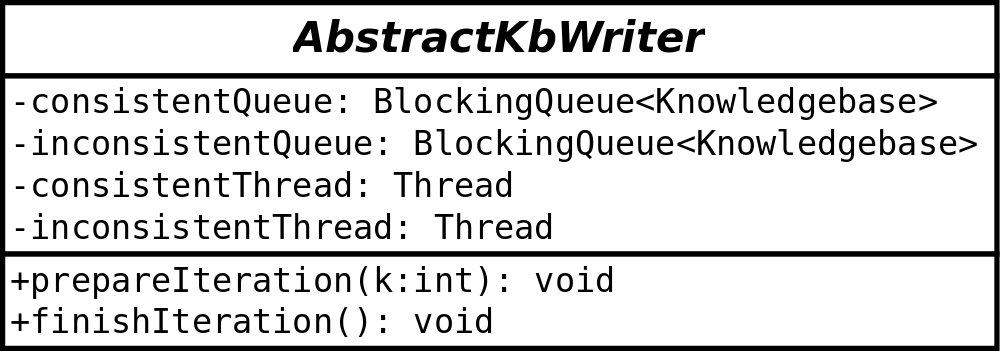
\includegraphics[width=0.45\linewidth]{bilder/AbstractKbWriter.png}
\caption{AbstractKbWriter}
\label{pic:abstractkbwriter}
\end{figure}


\textit{AbstractKbWriter} ist die abstrakte Klasse die von den beiden Varianten der Verarbeitung von Wissensbasen implementiert wird. Der Aufbau der Klasse AbstractWriter hat einige Ähnlichkeiten zur bereits beschriebenen Klasse AbstractPairWriter. Ein vereinfachtes Klassendiagramm ist in \autoref{pic:abstractkbwriter} zu sehen. Es gibt zwei BlockingQueues als Instanzvariablen. Eine \textit{consistentQueue}, in welche GenKB die konsistenten Wissensbasen einfügt und die \textit{inconsistentQueue} in der GenKB die inkonsistenten Wissensbasen einreiht. Die Beiden Queues werden auch direkt im Konstruktor des AbstractKbWriter als \textit{ArrayBlockingQueue(5000)} initialisiert. Für jede der beiden BlockingQueues existiert ein eigener Thread, der sich um die Bearbeitung der Queues kümmert. Hier also ein Thread für die konsistenten und ein Thread für die inkonsistenten Wissensbasen. Die beiden BlockingQueues ochestrieren hier also wieder die Zusammenarbeit von GenKB und den beiden Writer Threads. Zum Iterationswechsel sind auch hier zwei Methoden vorhanden, \textit{prepareIteration(int k)} zur Vorbereitung einer neuen Iteration und \textit{finishIteration()} zum korrekten Beenden der aktuellen Iteration. Der AbstractKbWriter ist weiterhin die Stelle im Programm, an welcher die generierten Wissensbasen gezählt werden. Um diese Information an die GUI weitezugeben, existieren die drei folgenden Getter: \textit{getTotalConsistentKbAmount()}, \textit{getTotalInconsistentKbAmount} und \textit{getIterationConsistentAmount()}.
Daneben gibt es noch im  oberen gezeigten Diagramm nicht erwähnte Methoden, um weitere Informationen an die GUI weiterzugeben: Das sind hier Getter für die aktuell belegte Größe der Queues und eine Methode um die Threads außerplanmäßig über den Stop Button zu beenden.

\subsubsection{KbFileWriter}
\label{sec:kbfilewriter}
Der \textit{KbFileWriter} ist diejenige Impelementierung von AbstractKbWriter, welche die Wissensbasen tatsächlich in Dateien schreibt und abspeichert. Die erstellen Dateien können mehrere Wissensbasen enthalten und werden mit der Dateiendung \glqq .cl\grqq \space gespeichert. Dazu besitzt der KbFileWriter zwei gleichermaßen aufgebaute Threads: Ein Thread für die \textit{consistentKbQueue} und ein Thread für die \textit{inconisstentKbQueue}. Die beiden Threads beobachten ihre zugeordnete Queue und sobald sich darin Elemente befinden, werden diese in eine Liste eingefügt. Wenn die Länge der Liste die maximale Anzahl an Wissensbasen erreicht hat, welche in der GUI bestimmt wird, wird die Liste auf den Speicher geschrieben. Dazu wird eine neue  Datei im Unterordner \glqq consistent\grqq \space oder \glqq inconsistent\grqq \space  und jeweils darin im Unterordnet der aktuellen Iteration $k$ erstellt. Zum Speichern der Wissensbasen stehen zwei Optionen bereit: Entweder wird ein Konditional nur durch dessen Nummer in die Datei geschrieben oder als kompletter String im InfOCF Format. Wenn eine Iteration beendet ist, wird die letzte Datei geschrieben welche entsprechend weniger Wissensbasen als die Anderen beinhalten kann. Da der KbFileWriter recht viele Optionen bietet, bekommt er von der GUI ein KbWriterOptions Objekt mit allen vom Benutzer gewählten Einstellungen um diese umzusetzen.\\
Beide Threads besitzen und aktualisieren zudem jeweils einen Zähler für die Gesamtmenge der Wissensbasen über alle Iterationen und für die aktuelle Iteration. Der Creator selbst hat keinen Zähler, die GUI holt sich die Information zum anzeigen aus dem AbstractWriter. Der Zweck den Zähler hier unterzubringen ist es, den Creator so weit wie möglich von nicht wirklich notwendigen Operationen zu entlasten um eine bestmögliche Geschwindigkeit zu ermöglichen.\\
Neben den Threads besitzt der KbFileWriter die Methode \textit{finishIteration()}, welche dafür sorgt, dass der aufrufende Thread (der Creator) so lange wartet, bis alle in der Queue vorhandenen Wissensbasen auch korrekt gespeichert und gezählt werden. Das löst insbesondere auch das Schreiben der restlichen Wissensbasen der Queue in die letzte Datei aus. Damit wird ein sauberer Abschluss einer Iteration gewährleistet. Die Methode \textit{newIteration(int k)} initialisiert dann die Threads für eine neue Iteration und legt die benötigten Unterordner an. \\
Der KBFileWriter bietet für das Schreiben von Dateien die Option an, eine feste minimale Länge der Dateinamen einzustellen, falls das gewünscht sein sollte. Dann werden die Namen bei Bedarf mit \textit{leading zeroes} aufgefüllt. Standardmäßig ist die Option deaktiviert in dem Sinne, dass die minimale Länge der Dateinamen auf 1 gesetzt ist. Wenn die Anzahl der Dateien (in einem Unterordner, also innerhalb einer Iteration) die Grenze dessen Überschreitet, was mit einer Zahl der definierten Länge dargestellt werden kann, werden die Zahlen einfach länger. Das ist das einfache Prinzip nach dem Motto: Nach 9 folgt 10. Der Benutzer muss sich die Länge entsprechend vorher überlegen oder einfach entsprechend große Werte wählen. 


\subsubsection{DummyKbWriter}
\label{sec:dummywriter}
Auch der DummyKbWriter besitzt zwei gleich aufgebaute Threads: Einer kümmert sich um die \textit{consistentKbQueue}, der Andere bearbeitet die \textit{inconsistentKbQueue}. Beide Threads beobachten ihre Queue und sobald Elemente darin erscheinen, werden diese gezählt und sofort wieder gelöscht. Das Zählen findet einmal  in Bezug auf die Gesamtmenge des Programmverlaufs über alle Iterationen statt und einmal auf die aktuelle Iteration. Die gezählten Werte ruft die grafische Oberfläche dann ab, um sie für den Benutzer anzuzeigen. Weiterhin besitzt der DummyKbWriter noch eine Methode zum Iterationswechsel, die macht allerdings nichts anderes als den Zähler der Wissensbasen für die aktuelle Iteration wieder auf 0 zu setzen.

\subsection{Grafische Oberfläche zum Generieren der Konditionale}


\begin{figure}
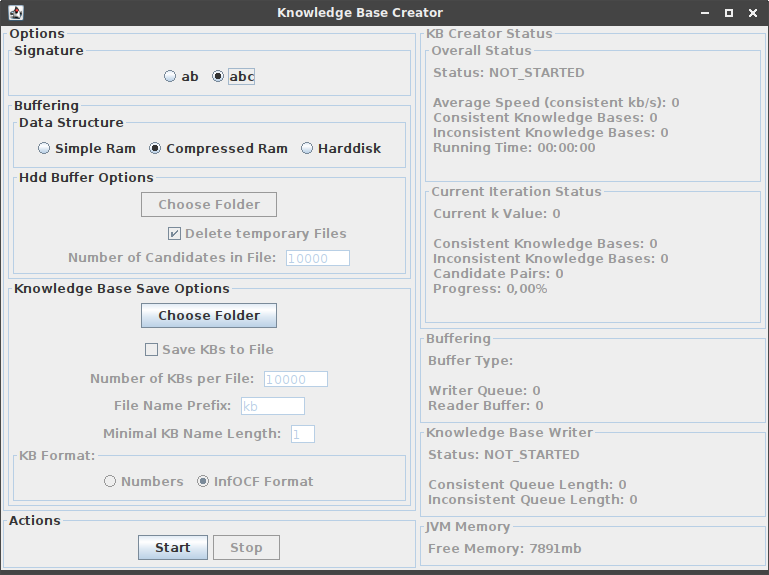
\includegraphics[width=0.97\linewidth]{bilder/KbCreator_screen.png}
\caption{Screenshot KbKreator GUI}
\label{pic:kbcreator_screen}
\end{figure}


Die Grafische Oberfläche des KBCreators ist in \autoref{pic:kbcreator_screen} gezeigt und besteht aus zwei Teilen: Die linke Seite beinhaltet die möglichen Optionen, die zum generieren der Wissensbasis eingestellt werden können. Einige Optionen sind dabei von Anderen abhängig und werden ausgegraut dargestellt, wenn sie in der aktuell eingestellten Situation nicht sinnvoll zu bearbeiten sind. Am unteren Ende der Einstellungen befinden sich der Start und der Stop Button für den KbCreator.\\
Auf der Rechten Seite befindet sich die Anzeige für den aktuellen Status mit vielen Details. Wenn der Creator nicht läuft, ist die gesamte rechte Seite ausgegraut. Wenn er läuft, werden die Informationen mit schwarzer Schrift dargestellt und laufend aktualisiert, die Aktualisierung übernimmt ein eigener Thread. Wenn der Creator gestoppt wird, wird die rechte Seite wieder ausgegraut. Die Informationen vom Zeitpunkt des Beenden des Creators werden jedoch weiterhin angezeigt. \\
Die Bedienung des KbCreators erfolgt ausschließlich über die GUI und nicht über das Terminal. Die meisten Informationen werden auch auf der GUI angezeigt. Im Terminal werden noch einige zusätzliche Informationen angezeigt, insbesondere zum Wechsel der Iterationen oder wenn unerwartete Fehler auftreten sollten.
\subsubsection{Optionen und Start}
Auf der linken Seite befinden sich die einstellbaren Optionen für den KBCreator. Ganz oben lässt sich die Signatur auswählen, als Optionen stehen \textit{ab} und \textit{abc} bereit. Default ist \textit{abc}. Im zweiten Abschnitt wird das Buffering gewählt, also die konkrete Vairante zur Zwischenspeicherung der Daten während des Programmablaufs wie unter \autoref{sec:pairbuffer} beschrieben. Es stehen die drei dort vorgestellten Varianten zur Verfügung. Die Voreingestellung ist der CompressedRamBuffer. Weiterhin möglich ist auch der SimpleRamBuffer. Wenn hier der Radiobutton für \textit{Harddisk} ausgewählt wird, wird das darunterliegende Panel freigeschaltet. Dort befinden sich die genaueren Einstellungen für die Zwischenspeicherung auf der Festplatte. Zum einen lässt sich dann der Ordner auswählen, in dem die Daten zwischengespeichert werden. Hier kann der selbe Ordner ausgewählt werden wie zum Speichern der Wissensbasen selbst denn es werden automatisch Unterordner erzeugt sodass sich die Daten nicht vermischen würden. Darunter befindet sich eine standardmäßig aktivierte Checkbox, die das automatische löschen der temporären Dateien einstellt. Wird das Häkchen entfernt, werden die temporären Daten nicht automatisch gelöscht und können vom Benutzer betrachtet werden. Als dritte Option kann die Menge der Paare $<R,C>$ aus Wissensbasen und Kandidaten eingestellt werden, die zusammen in einer Textdatei gespeichert werden. Hohe Werte sind hier sinnvoll, damit keine zu großen Mengen an kleinen Dateien geschrieben und wieder gelöscht werden müssen. \\
Darunter befinden sich die letzte Kategorie der Optionen mit dem Einstellungen zum Speichern der Wissensbasen. Ganz oben kann ein Ordner ausgewählt werden, in dem die Wissensbasen gespeichert werden. Für die Wissensbasen wird dann automatisch ein Unterordner erstellt und weitere Unterordner für die Iterationen $k$. Wenn ein gültiger Ordner ausgewählt ist wird als Option zum Speichern der \textit{KbFileWriter} wie in \autoref{sec:kbfilewriter} beschrieben aktiviert und die weiteren Optionen zum Speichern freigeschaltet. Wird kein Ordner ausgewählt, werden die Wissensbasen nicht gespeichert und es wird die Option \textit{DummyWriter} wie in \autoref{sec:dummywriter} beschrieben verwendet. Für das Zwischenspeichern der Daten stehen folgende Optionen bereit: Erstens die Checkbox, dass die Daten gespeichert werden sollen. Mit ihr kann einmal eingestelltes Speichern wieder deaktiviert werden. Als nächstes Kann die Anzahl der Wissensbasen eingestellt werden, die pro Datei abgespeichert werden soll. Danach kann ein Präfix für die namen Wisensbasen selbst  und die Dateinamen vergeben werden. Wenn Beispielsweise hier \glqq kb\grqq \space eingetragen wird, werden die Wissensbasen nach dem Schema \glqq kb + [laufende Nummer]\grqq \space vergeben. Die Dateinamen erhalten dann das Präfix ebenfalls. Darunter kann mit der Option "Minimal KB Name Length" eine Mindestlänge für die Namen der Wissensbasen und indirekt auch für die Namen der Dateien eingestellt werden. Voreingestellt ist der Wert 1, damit ist die Option praktisch deaktiviert. Wird beispielsweise 3 eingestellt, erhält die erste Wissensbasis den Namen \glqq 001\grqq . In der letzten Option kann per RadioBox eingestellt werden, ob die Wissensbasen nur als Nummer oder als InfOCF String in die Datei geschrieben werden Voreingestellt ist der InfOCF String.\\
Ganz unten befinden sich die Buttons für Start und Stop. Von den Buttons ist jeweils nur der aktuell sinnvolle aktiviert und der andere ausgegraut. Mit \glqq Start \grqq \space werden die aktuell eingestellten Optionen verwendet und die Generierung der Wissensbasen beginnt. Das betätigen von Start deaktiviert graut auch alle Einstellmöglichkeiten aus. Die Einstellungen selbst bleiben jedoch bestehen, sodass man diese später auch bei Bedarf noch angesehen kann. Mit drücken des Buttons \glqq Stop\grqq \space kann die Generierung wieder gestoppt werden.
\subsubsection{Statusanzeige}
Auf der Rechten Seite werden Informationen zum Programmstatus angezeigt, während der KBCreator läuft. Sie sind jeweils unter verschiedenen Kategorien gruppiert. Im Folgenden werden die Kategorien von oben nach unten erklärt. \\
Ganz oben befindet sich der OverallCreatorStatus. Hier wird der Status des KbCreator selbst in der ersten Zeile angezeigt. Mögliche Werte sind hierfür: NOT$\_$STARTED, RUNNING, STOPPED und FINISHED. Danach folgen einige Informationen zum aktuellen Programmablauf über alle Iterationen hinweg. Angezeigt werden: die Durchschnittsgeschwindigkeit (In konsistente Wissensbasen pro Sektunde über dem gesamten Programmablauf) und die Gesamtmenge der erstellten konsistenten und inkonsistenten Wissensbasen. Ebenfalls wird die Zeit angezeigt, seitdem der KbCreator schon läuft. \\
Im nächsten Abschnitt werden Informationen zur aktuellen Iteration $k$ angezeigt. Das ist zu ganz oben der aktuelle Wert für $k$ selbst. Danach die generierte Mengen an konsistenten und inkonsistenten Wissensbasen in der aktuellen Iteration. Darunter die Angabe \glqq Candidate Pairs\grqq \space. Sie beschreibt die Gesamtmenge an Paaren $<R, C>$ aus Kandidaten und Wissensbasen, die in dieser aktuellen Iteration bearbeitet werden müssen. Zum Schluss eine Fortschrittsanzeige in Prozent: Sie zeigt den momentanen Fortschritt der aktuellen Iteration. Dieser Wert errechnet sich aus dem Anteil der schon bearbeiteten Paare $<R,C>$ von der gesamtMenge der dieser Paare. Dadurch steigt der Prozent Wert in einer Iteration erst rechtn langsam, dann immer schneller. Das liegt daran, dass zuerst zeitintensiv diejenigen Paare mit einer großen Anzahl von Kandidaten bearbeitet werden, was entsprechend länger dauert. daher steigt dieser Wert zum Ende einer Iteration immer schneller an. \\
Darunter befinden sich Informationen zum Buffering. Erstens der zuvor ausgewählte BufferType selbst, also SIMPLE$\_$RAM, COMPRESSED$\_$RAM oder HDD. Darunter befinden sich die Queues \textit{NewIterationQueue} und \textit{lastIterationQueue} wie in \autoref{sec:abstractbuffer} beschrieben. \\
Als nächstes folgen Informationen zum KnowledgeBaseWriter. Erstens der aktulle Status Status als NOT$\_$STARTED, RUNNING und DUMMY$\_$WRITER. Darunter der aktuelle Füllstand der Queues für konsistente und inkonsistente Wissensbasen. \\
Ganz unten befindet sich eine Information zur Java JVM selbst: Sie gibt im Prinzip den noch freien Arbeitsspeicher an. Diese Information ist etwas erklärungsbedürftig: Der Wert beschreibt in etwa den noch freien HEAP der JVM in Megabytes. Das ist also der Platz, der für neu erstellte Objekte noch zur Verfügung steht. Möglicherweise kann der GarbageCollector jedoch bei bedarf noch etwas mehr Speicher zur Verfügung stellen. Der Wert ist also überhaupt nicht präzise, trotzdem ein guter Anhaltspunkt zum Status des aktuellen Programmablaufs. Man kann zumindest einschätzen, ob noch Speicher frei ist, oder ob der Speicher voll ist. Konkret wird der Wert auf mit folgender Codezeile ermittelt:


%\begin{figure}
\begin{lstlisting}
(Runtime.getRuntime().maxMemory()-Runtime.getRuntime().totalMemory()) / 1_000_000
\end{lstlisting}


\section{Bewertung der Ergebnisse}
\subsection{Allgemein}
Als Ergebnis erzeugt das erstellte Programm Wissensbasen im gewünschten Format, sodass sie mit der InfOCF Bibliothek korrekt gelesen werden können. Die Wissensbasen werden nach Iterationen k gruppiert in Unterordnet abgespeichert. Das lässt sich leicht überprüfen da in einer Iteration k jede Wissensbasis genau $k+1$ Konditionale beinhaltet. Innerhalb der Iterationen werden die Wissensbasen nach konsistent und inkonsistent gruppiert. Die Korrektheit dieser Gruppierung lässt sich durch einlesen mit der InfOCF Bibliothek und Prüfen mit dessen Methode auf Konsistenz bestätigen. Des weiteren werden die Wissensbasen genau in der Reihenfolge, wie sie durch GenKB erzeugt werden, abgespeichert. Dafür sorgt die Verwendung von threadsicheren BlockingQueues. \\
Durch die Möglichkeit Speicherung der Daten zwischen zwei Iterationen auf der Festplatte ist dafür kein großer Arbeitsspeicher nötig. Der Algorithmus kann so sehr lange laufen und viele Wissensbasen erzeugen. Begrenzend könnte irgendwann der Platz auf der Festplatte werden. Aufgrund der enormen Menge der möglichen Wissensbasen werden mit der Signatur $\Sigma_{abc}$ nur sehr geringe Werte für k erreicht. Bei entsprechend langer Laufzeit sollte $k=3$ möglich sein, höhere Werte würden wohl zu lange dauern. Der Begrenzende Faktor ist die Geschwindigkeit des Prozessors. Teilweise kann durch Threading die Arbeit auf mehrere Kerne verteilt werden. Der Flaschenhals ist jedoch der Thread der GenKB selbst umsetzt.\\
Das ließe sich durch Multi Threading lösen. Ein Ansatz für GenKB mit Multi Threading wurde während der Entwicklung des beschriebenen Programms ausprobiert. Das parallele Erzeugen der Wissensbasen mit einem ExecutorService und mehreren Threads hat auch funktioniert. Im getesteten Threading wurden die Zeilen 9-12 von GenKb auf verschiedene Threads verteilt und dort bearbeitet. Gescheitert ist es jedoch am Speichern der Ergebnisse in der Reihenfolge wie sie der ursprüngliche Algorithmus vorgibt. Die Ergebnisse der parallelen Threads müssten dann nämlich wieder genau in der richtigen Reihenfolge eingesammelt werden. Mit einem von vornherein auf Multi Threading ausgerichtetem Design dürfte es aber möglich sein, mehrere Prozessorkerne für den Hauptalgorithmus zu nutzen und die Geschwindigkeit dadurch zu steigern. Dazu müsste das Design des Programmes jedoch grundsätzlich neu konzipiert werden.

\subsection{Programmablauf mit Signatur ab}
Mit der Signatur $\Sigma_{abc}$ kann das Programm tatsächlich alle Wissensbasen generieren. Dabei entstehen 364.144.824 konsistente und 364.304.482 inkonsistente Wissensbasen in 25 Iterationen. Die Wissensbasen als Ergebnis benötigen 257.1 GB Festplattenspeicher, der ganze Vorgang hat auf dem Test PC 1 Stunde und 52 Minuten gedauert. Dabei wurde die Zwischenspeicherung der Daten im Arbeitsspeicher des PCs verwendet. Der JVM mussten dafür mindestens 23 GB RAM zugewiesen werden. \\
Der Verlauf dieses Programmablaufs verlief etwa, wie man es erwarten sollte: Die ersten Iterationen laufen sehr schnell. Mit steigendem k steigt dann die Menge der Paare pro Iteration. Das Maximum ist bei $k=13$ mit 58,3 Paaren erreicht, danach sinkt die Anzahl wieder. Dadurch sinkt die Geschwindigkeit deutlich. Dazu kommt, dass mit steigendem $k$ die Prüfung der Wissensbasen auf Konsistenz länger dauert, wodurch sich die Dauer der Iterationen ebenfalls mit steigendem $k$ erhöht.


\subsection{Programmablauf mit Signatur abc}

Mit der Signatur sind erwartungsgemäß nur sehr geringe Werte für $k$ erreichtbar. Die erste Iteration $k=0$ ist unproblematisch, da hier nur die Wissensbasen mit jeweils einem Element erstellt werden. Entsprechend entstehen als Output 2774 konsistente und 0 inkonsistente Wissensbasen in weniger als einer Sekunde. \\
Die Iteration für $k = 1$ ist auf dem Test PC noch problemlos ohne Zwischenspeicherung der Daten auf der Festplatte durchführbar. Die dafür benötigte Zeit betrug 266 Sekunden. Als Ergebnis entstehen 7.975.405 konsistente und 210200 inkonsistente Wissensbasen. Im durchschnitt wurden also ca. 30.000 konsistente Wissensbasen pro Sekunde erstellt. Die gespeicherten Wissensbasen als Ergebnis benötigen dann etwa 1,1 GB Speicher, abhängig davon wie viele Wissensbasen man pro Datei schreiben lässt. \\
Die Iteration $k = 2$ für die 3 Elementen enthaltenden Wissensbasen wurde auf dem Test PC nicht vollständig durchgeführt. Sie dürfte auf jeden Fall um ein vielfaches mehr Speicher und Zeit benötigen, als die Iteration davor. Mit genügend Zeit und Festplattenspeicher sollte die Menge der Konditionale jedoch berechnet werden können. \\
Eine Prognose für die Laufzeit und den Speicherbedarf zu erstellen ist nicht zuverlässig möglich. Hier soll exemplarisch ein Versuch der Prognose für $k=2$ versucht werden. Dazu wird der Anfang der Iteration hochgerechnet, basierend auf den Prozentwert des Fortschritts, den die GUI anzeigt. Dabei entstehe aber das Problem, dass die ersten Prozente einer Iteration viel umfangreicher sind als die letzten Prozente, denn am Anfang befinden sich die Paare mit vielen Kandidaten und am ende die Paare mit wenigen Kandidaten. Der Fortschritt wird jedoch basierend auf dem Anteil der bereits bearbeiteten Paare von der Gesamtmenge der Paare angezeigt. Wenn man also den Anfang einer Iteration auf den Rest extrapoliert, wird man den Umfang einer Iteration deutlich überschätzen. Die Information in der Extrapolation liegt in einer oberen Grenze, die sicher deutlich unterschritten wird. Unklar ist, wie viel die Ergebnisse unterschritten werden. \\
Als Basis für die Prognose wurde die Iteration $k=2$ bis zum Fortschritt von 0.05 $\%$ als Stichprobe betrachtet. Das tatsächliche Ergebnis könnte also das 2000 fache der Ergebnisse nicht überschreiten und wird sicher deutlich darunter liegen. Als Optionen dafür war das zwischenspeichern der Daten im Arbeitsspeicher aktiv und die Wissensbasen wurden im InfOCF Format auf die Festplatte geschrieben. Die Messwerte beziehen sich dabei \textit{nur} auf den Teil, der auf Iteration $k=2$ fällt. Als Ergebnis wurden eine Zeit von 9 Minuten gemessen. Dabei wurden ca. 14.700.000 konsistente und 650.000 inkonsistente Wissensbasen erstellt. Der Arbeitsspeicher der JVM (7 GB) kam dabei an seine Grenzen aber reichte noch aus. Zum speichern der Wissensbasen wurden 2,4 GB benötigt. Als absolute Obergrenze für diese Iteration ergeben sich nun 29.400.000.000 (also 29,4 Milliarden) konsistente und 1.300.000.000 (1,3 Mrd) inkonsistente Wissensbasen. Dafür könnten 12,5 Tage und 4,8 TB Festplattenspeicher benötigt werden. Wie gesagt, diese Werte sind absolute Obergrenzen, die realen Werte werden deutlich darunter liegen.


\subsection{Betrachtung von Knowledge Base Creator mit JVisualVM}

In diesem Abschnitt soll kurz die Betrachtung des Erstellten Programms mit dem Profiler JVisualVM gezeigt werden. JVisualVM ist ein Profiler, mit dem Java Programme während der Laufzeit näher betrachtet werden können, siehe dazu auch \cite{jvis20}. Mit diesem Tool lassen sich insbesondere Informationen zum Speicherverbrauch und zur CPU Nutzung von Java Anwendungen finden. Es lassen sich weiterhin Details zu laufenden Threads und zur Rechenzeit einzelner Methoden untersuchen. \\
Bei einer Anwendung des Profilers auf KbCreator zeigt sich wie erwartet, dass der GenKb Thread mit Abstand am meisten CPU Zeit benötigt. Dieser Thread ist also der Flaschenhals im Programm und hier müsste man ansetzen, wenn der Ablauf beschleunigt werden soll. Im GenKb Thread selbst ist erwartbar die \textit{isConsistentWith(Conditional)} Methode der Klasse Knowledgebase die Stelle, an der am meisten Rechenzeit verbraucht wird. \\
Beim Arbeitsspeicherverbrauch wird hier nur der Programmablauf mit Zwischenspeicherung der Daten im Arbeitsspeicher betrachtet, da der Speicher ansonsten keine kritische Stelle darstellt. Hier entfällt der größte Teil des Speichers (ca. 30$\%$) auf \textit{java.lang.Object[]}, also Arrays von Objekten. Das sind sicherlich zum Großteil die List<List<AbstractPair>> Objekte, die intern mit einer ArrayList arbeiten und die Paare zwischen den Iterationen speichern. Der zweite große Block (ca. 15$\%$) entfällt auf Arrays von \textit{int} Werten. Das dürften die komprimierten Kandidatenarrays in den \textit{CompressedPairs} sein. Ansonsten belegen noch Instanzen von \textit{ArrayList}, \textit{KnowledgeBase} und \textit{CompressedPair} jeweils ca. 10 $\%$ des Hauptspeichers. \\
Die Betrachtung des Threadings mit dem Profiler bestätigt ansonsten naheliegende Erwartungen. Über die verschiedenen Iterationen werden diverse Threads neu gestarted und auch wieder korrekt beendet. Ansonsten sind keine Auffälligkeiten zu beobachten.




\newpage

\section*{Abbildungsverzeichnis}
Alle Abbildungen in diesem Dokument sind eigene Darstellungen. Die Klassendiagramme wurden mit der Sofware \glqq Dia\grqq \space erstellt. Die schematischen Darstellungen zum Überblick über das erstellte Programm sind ebenfalls mit der Software \glqq Dia\grqq \space erstellt. Screenshots  wurden mit dem Programm \glqq Xfce4-Screenshooter \grqq \space erstellt.
\bibliography{lit} 
\end{document}